\documentclass{patmorin}
\listfiles
\usepackage{amsthm,amsmath,graphicx,wrapfig}
\usepackage{pat}
%\usepackage{coffee4}
\usepackage[letterpaper]{hyperref}
\usepackage[dvipsnames]{color}
\definecolor{linkblue}{named}{Blue}
\hypersetup{colorlinks=true, linkcolor=linkblue,  anchorcolor=linkblue,
citecolor=linkblue, filecolor=linkblue, menucolor=linkblue, pagecolor=linkblue,
urlcolor=linkblue} \setlength{\parskip}{1ex}

\usepackage[skip=0pt]{caption}

\newcommand{\lstlabel}[1]{\label{lst:#1}}
\newcommand{\lstref}[1]{Listing~\ref{lst:#1}}
\newcommand{\Lstref}[1]{\lstref{#1}}

\newcommand{\naive}{na\"{\i}ve}

\usepackage{listings}
\usepackage{minted}
\usepackage{mdframed}
\surroundwithmdframed{minted}

\title{\MakeUppercase{Array Layouts for Comparison-Based Searching}\thanks{This research is partially funded by NSERC.}}
\author{Paul-Virak Khuong\footnote{AppNexus, \email{pvk@pvk.ca}}\,\, 
    and Pat Morin\footnote{Carleton University, \email{morin@scs.carleton.ca}}}


\begin{document}
\begin{titlepage}
\maketitle


\begin{abstract}
  We attempt to determine the best order and search algorithm to store
  $n$ comparable data items in an array, $A$, of length $n$ so that we
  can, for any query value, $x$, quickly find the smallest value in $A$
  that is greater than or equal to $x$. In particular, we consider the
  important case where there are many such queries to the same array,
  $A$, which resides entirely in RAM.  In addition to the obvious sorted
  order/binary search combination we consider the Eytzinger (BFS) layout
  normally used for heaps, an implicit B-tree layout that generalizes
  the Eytzinger layout, and the van Emde Boas layout commonly used in
  the cache-oblivious algorithms literature.

  After extensive testing and tuning on a wide variety of modern hardware,
  we arrive at the conclusion that, for small values of $n$, sorted
  order, combined with a good implementation of binary search is best.
  For larger values of $n$, we arrive at the surprising conclusion that
  the Eytzinger layout is usually the fastest.  The latter conclusion is
  unexpected and goes counter to earlier experimental work by Brodal,
  Fagerberg, and Jacob (SODA~2003), who concluded that both the B-tree
  and van Emde Boas layouts were faster than the Eytzinger layout for
  large values of $n$.
\end{abstract}

\end{titlepage}

\pagenumbering{roman}
\tableofcontents
\newpage

\pagenumbering{arabic}
\section{Introduction}

A sorted array combined with binary search represents \emph{the} classic
data structure/query algorithm pair: theoretically optimal, fast in
practice, and discoverable by school children playing guessing games.
Although sorted arrays are \emph{static}---they don't support efficient
insertion or deletion---they are still the method of choice for bulk or
batch processing of data. Even \naive\ implementations of binary search
execute searches several times faster than the search algorithms of most
popular dynamic data structures such as red-black trees.\footnote{For
example, Barba and Morin \cite{barba.morin:top-down} found that a \naive\
implementation of binary search in a sorted array was approximately
three times faster than searching using C++'s \texttt{stl::set} class
(implemented as a red-black tree).}

It would be difficult to overstate the importance of
algorithms for searching in a static sorted set.
Every major programming language and environment provides a sorting
routine, so a sorted array is usually just a function call away. Many
language also provide a matching binary search implementation.
For example, in C++, sorting is done with \mintinline{c++}{std::sort()}
and the binary search algorithm is implemented in \mintinline{c++}{std::lower_bound()}
and \mintinline{c++}{std::upper_bound()}.
Examples of binary search in action abound; here are two:

\begin{enumerate}
\item The Chromium browser code-base
calls \mintinline{c++}{std::lower_bound()} and
\mintinline{c++}{std::upper_bound()} from 135 different locations
in a wide variety of contexts, including cookie handling, GUI
layout, graphics and text rendering, video handling, and certificate
management.\footnote{\url{https://goo.gl/zpSdXo}} This is the source code
that is built and packaged to make Google Chrome, a web browser that has more than a billion users \cite{protalinksi:google}.

\item Repeated binary searches in a few sorted arrays
represent approximately 10\% of the computation time for the AppNexus
real-time ad bidding engine. This engine runs continuously on 1500 machines
and sees 80\% of traffic on the internet.
\end{enumerate}

However, sorted order is just one possible layout that can be used to
store data in an array. Other layouts are also possible and---combined
with the right query algorithm---may allow for faster queries.
Other array layouts may be able to take advantage of (or be hurt less
by) modern processor features such as caches, instruction pipelining,
conditional moves, speculative execution, and prefetching.

  
In this experimental paper we consider four different memory layouts and
accompanying search algorithms.  The following points describe the scope of our study:

\begin{itemize}
\item We only consider array layouts that store $n$ data items in a
      single array of length $n$.

\item The search algorithms used for each layout can find (say) the
      index of the largest value that is greater than or equal to $x$
      for any value $x$. In case $x$ is greater than any value in the
      array, the search algorithm returns the index $n$.

\item We study real (wall-clock) execution time, not instruction counts,
      branch mispredictions, cache misses, other types of efficiency,
      or other proxies for real time.

\item We ignore the time required to construct the array
      layout.\footnote{All four layouts can be constructed in $O(n)$
      time given a sorted array.  Though we don't report construction
      times in the current paper, they are included in the accompanying
      data sets.  For all layouts it is faster to construct a layout for an
      array of size $10^8$ than it is to perform $2\times10^6$ searches
      on the resulting layout.}
\end{itemize}

We consider the following four layouts (here and throughout, $\log
n=\log_2 n$ denotes the binary logarithm of $n$):

\begin{enumerate}
  \item \texttt{Sorted}:  This is the usual sorted layout, in which
  the data is stored in sorted order and searching is done using binary
  search.

  \item \texttt{Eytzinger} (see \figref{eytzinger}): In this layout,
  the data is viewed as being stored in a complete binary search tree and
  the values of the nodes in this virtual tree are placed in the array in
  the order they would be encountered in a left-to-right breadth-first
  traversal.  The search algorithm simulates a search in this implicit
  binary search tree.

  \begin{figure}
    \begin{center}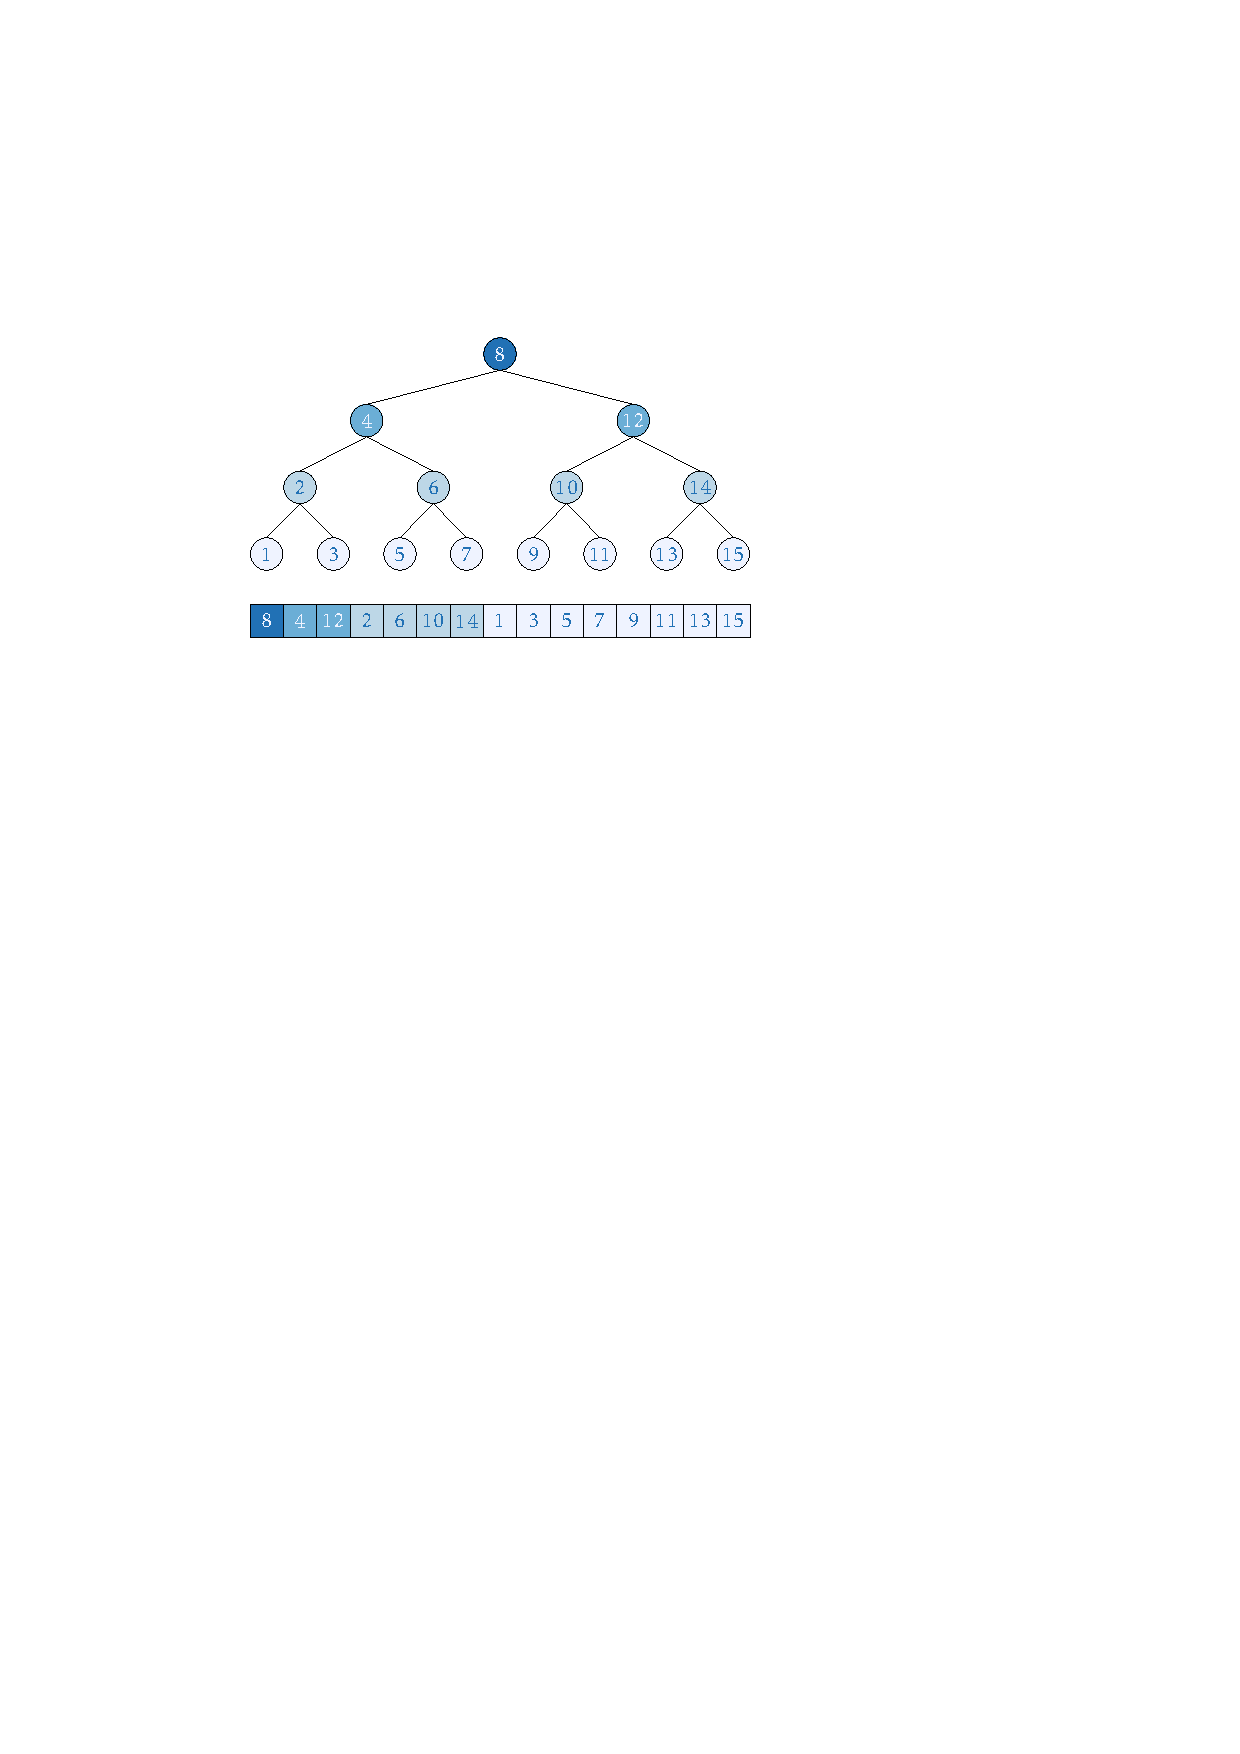
\includegraphics{eytzinger}\end{center}
    \caption{The Eytzinger layout}
    \figlabel{eytzinger}
  \end{figure}

%  The root of this tree is
%  stored at $A[0]$, and the left and right children of the node stored
%  at $A[i]$ are stored at $A[2i+1]$ and $A[2i+2]$, respectively.

  \item \texttt{Btree} (see \figref{btree}): In this layout, the data is
  viewed as being stored in a complete $(B+1)$-ary search tree, so that each
  node---except possibly one leaf---stores $B$ values.  The parameter
  $B$ is chosen so that $B$ data items fit neatly into a single cache line
  and the nodes of this tree are mapped to array locations in the order
  they are encountered in a breadth-first search.

  \begin{figure}
    \begin{center}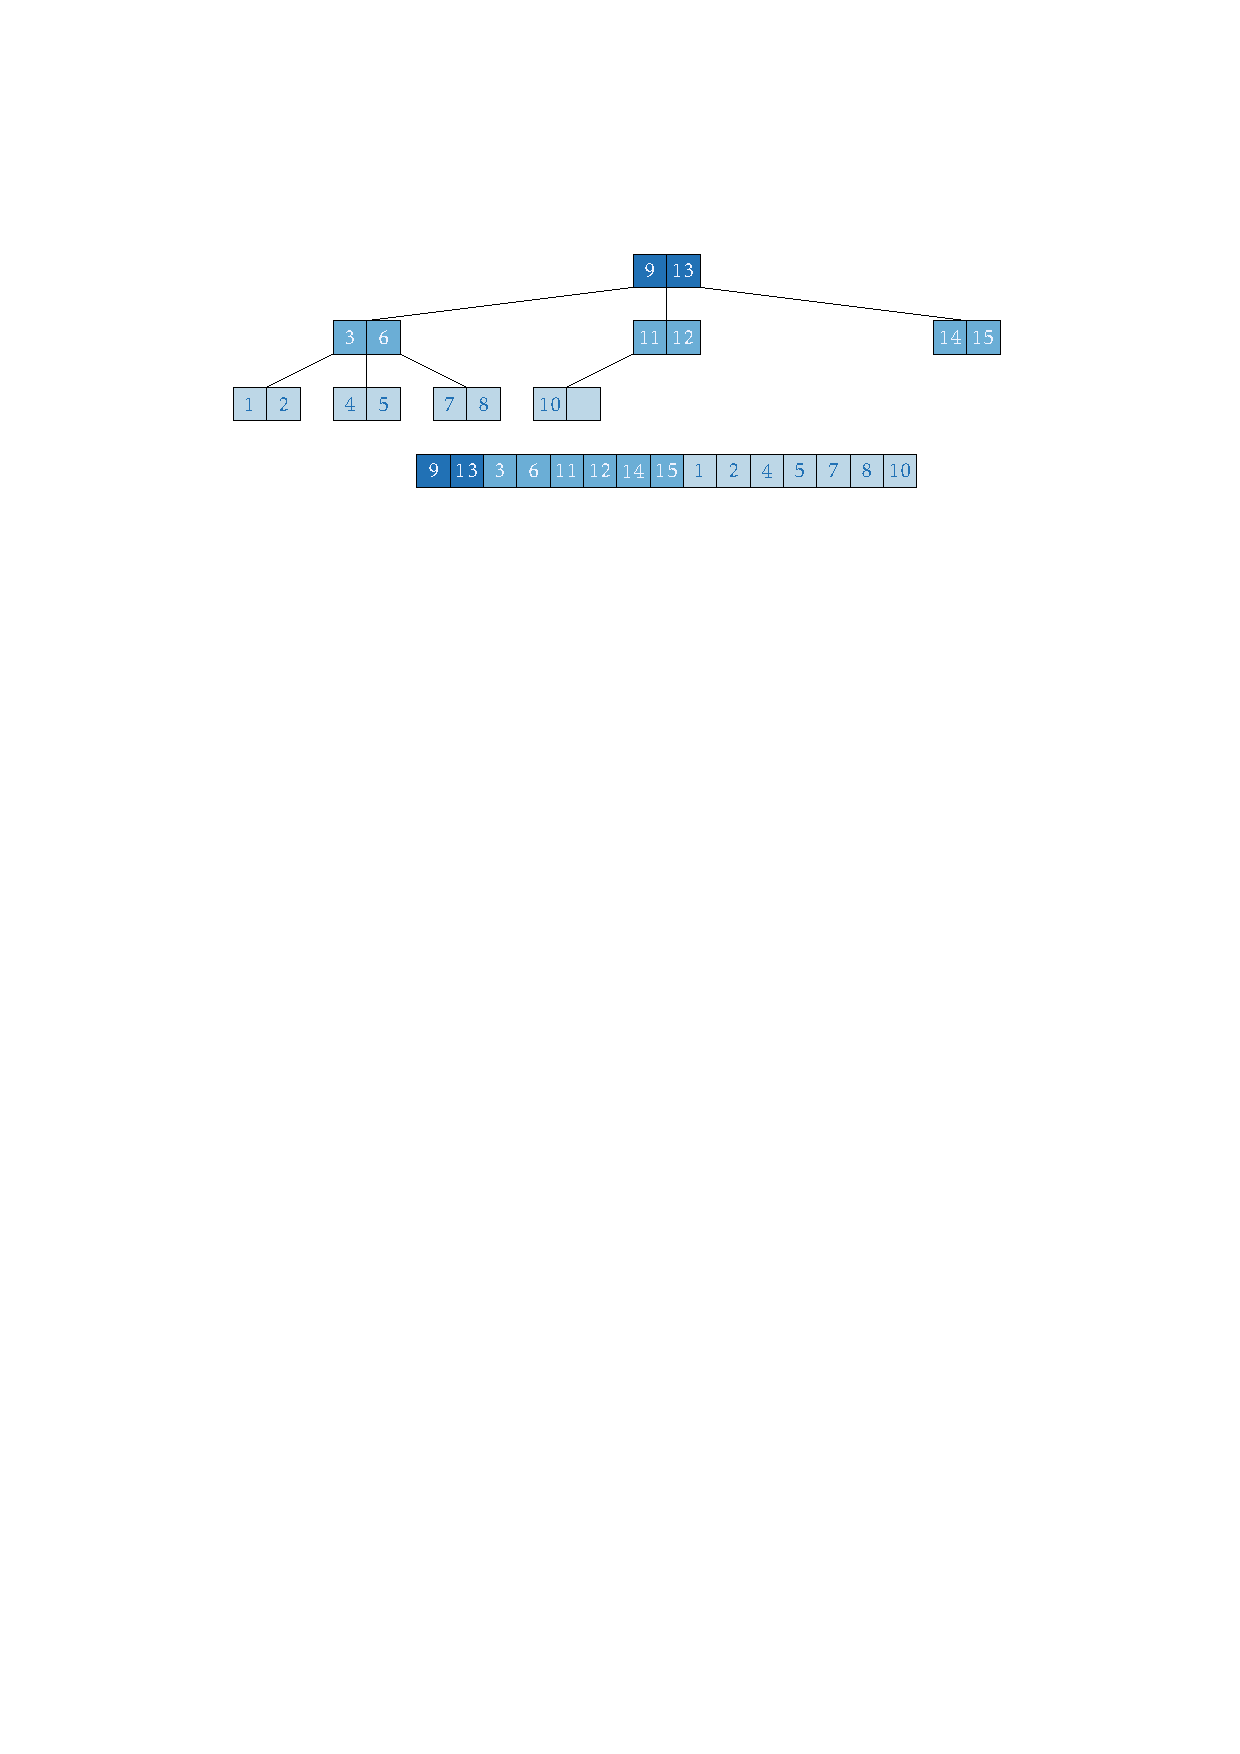
\includegraphics{btree}\end{center}
    \caption{The Btree layout with $B=2$}
    \figlabel{btree}
  \end{figure}

%  using
%  a generalization of the Eytzinger mapping:  For $j\in \{0,\ldots,b\}$,
%  the $j$th child of the node that starts at position $i$ is stored
%  beginning at position $i(b+1)+(j+1)b$.

  \item \texttt{vEB} (see \figref{veb}): In this, the \emph{van Emde
  Boas} layout, the data is viewed as being stored in a complete binary
  tree whose height is $h=\lceil\log (n+1)\rceil -1$. This tree is
  laid out recursively:  If $h=0$, then the single node of the tree
  is stored in $A[0]$.  Otherwise, the tree is split into a top-part
  of height $\lfloor h/2\rfloor$, which is recursively laid out in
  $A[0,\ldots,2^{1+\lfloor{h/2\rfloor}}-2]$.  Attached to the leaves of
  this top tree are up to $2^{1+\lfloor{h/2\rfloor}}$ subtrees, which
  are each recursively laid out, in left-to-right order, starting at
  array location $A[2^{1+\lfloor{h/2\rfloor}}-1]$.

  \begin{figure}
    \begin{center}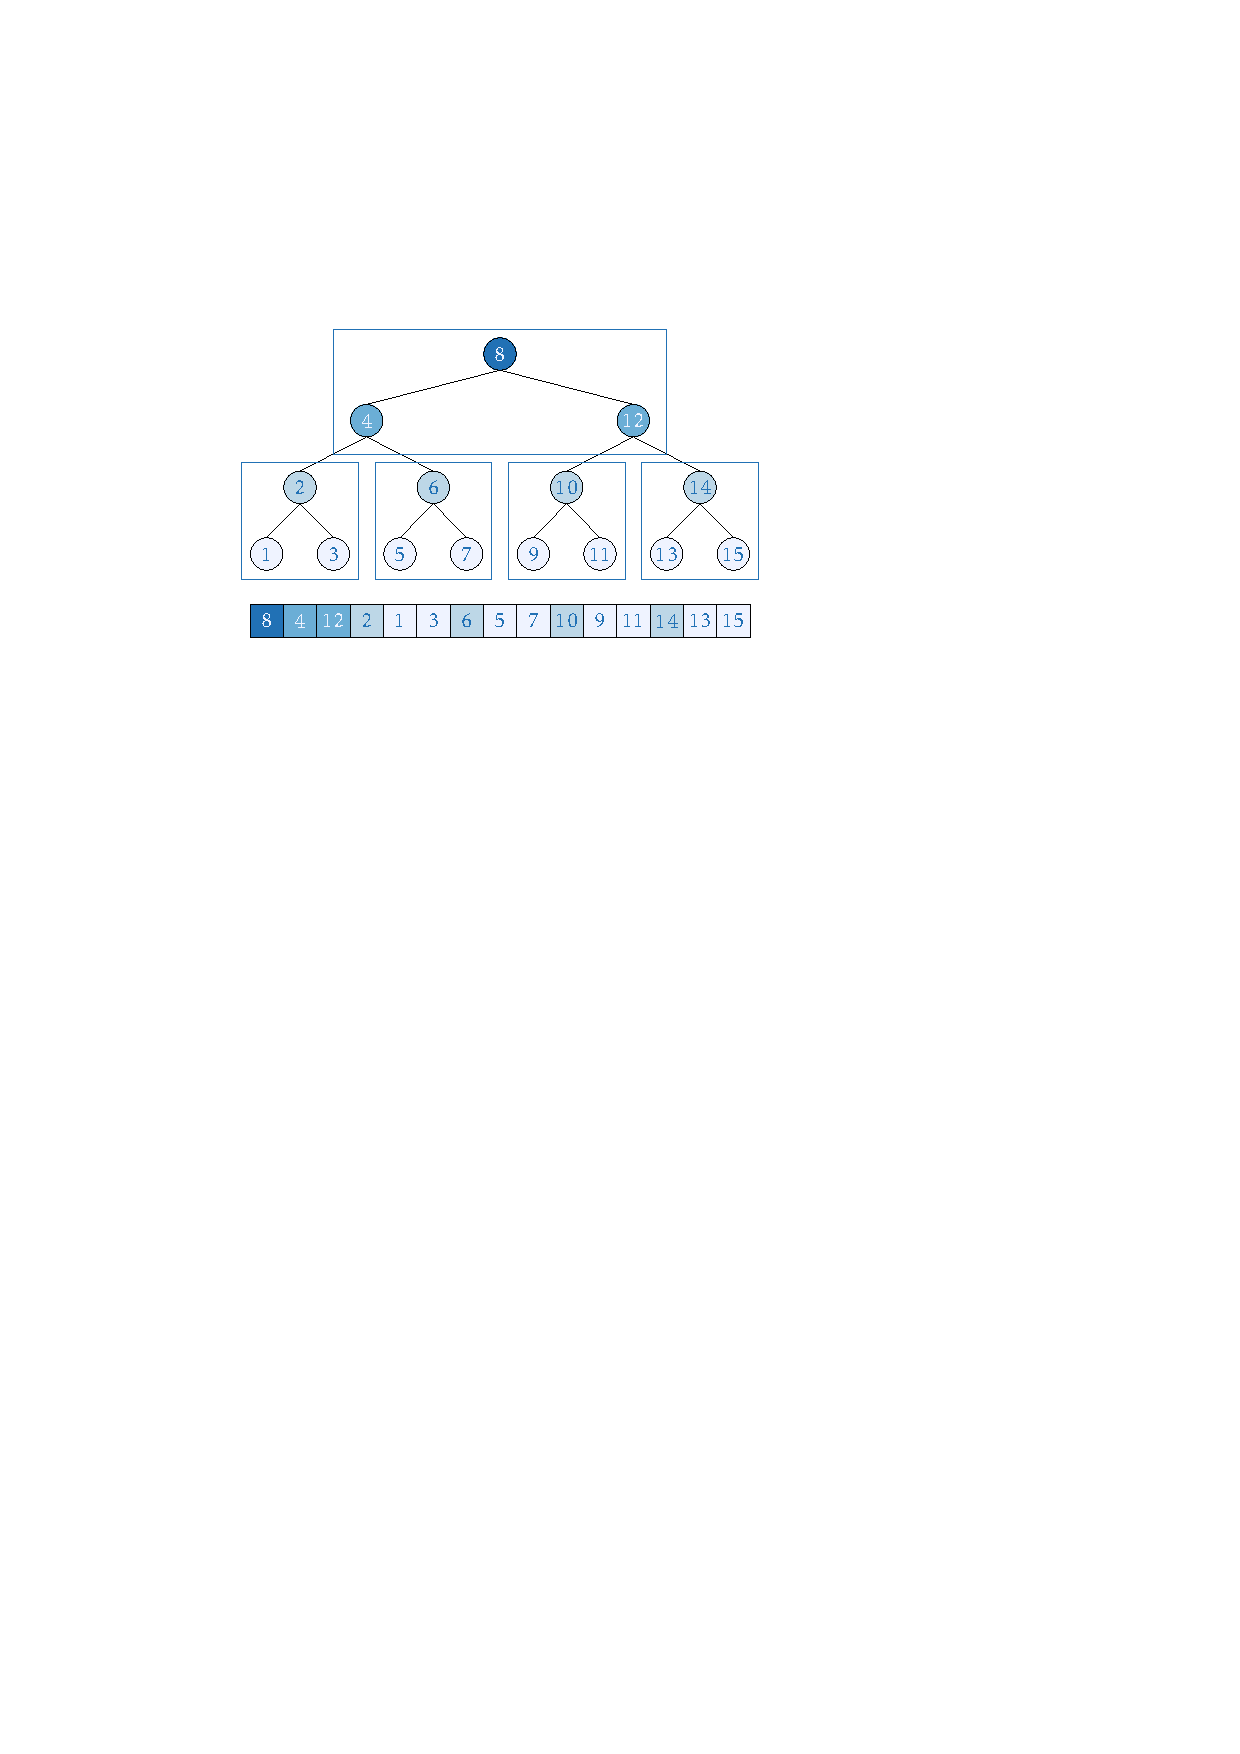
\includegraphics{veb}\end{center}
    \caption{The vEB layout}
    \figlabel{veb}
  \end{figure}


\end{enumerate}

\subsection{Related Work}

Of the four memory layout/search algorithm pairs we study, the sorted
array combined with binary search is, of course, the most well-known
and variants of binary search have been studied for more than half a
century. Knuth \cite[Section~6.2.1]{knuth:art} is a good reference.

The idea of implicitly representing a complete binary tree by listing
its nodes in breadth-first order goes back half a millenium to Eytzinger
\cite{eytzinger:thesaurus}. In more modern times, this method was proposed by
Williams for an implementation of binary heaps \cite{williams:algorithm}.

The implicit Btree layouts we study are a marriage of the Eytzinger
layout mentioned above and complete $(B+1)$-ary trees. This layout
was studied by Jones \cite{jones:empirical} and LaMarca and Ladner
\cite{lamarca.ladner:influence} in the context of implementing heaps.
Niewiadomski and Amaral \cite{niewiadomski.amaral:chopping} consider
an implicit $k$-ary heap implementation in which each node is itself
represented using hte Eytzinger layout.

The vEB layout was proposed by Prokop
\cite[Section~10.2]{prokop:cache-oblivious} because it has the advantage
over the Btree layout of being \emph{cache-oblivious}; the number of
cache lines used during a search is within a factor of four of what can
be obtained with a B-tree using an optimal choice of $B$.

%The effects of memory layouts on the performance of algorithms have been
%studied in other contexts as well. For example, for storing matrices,
%memory layouts have profound effects on the running times of various
%matrix operations \cite{X}.

The work most closely related to ours is that of Brodal, Fagerberg,
and Jacob \cite{brodal.fagerberg.ea:cache}. As part of their work on
cache-oblivious search trees, they present experimental results for
all four of the layouts we study here.  Based on their experiments,
they reach the following conclusions:

\begin{enumerate}

\item For array lengths smaller than the cache size, the layouts with
simplest address arithmetic---sorted and Eytzinger---were the fastest. The
Btree layout was next and the vEB layout, with its complicated address
arithmetic, was by far the slowest.

\item For array lengths much larger than the cache size, Btree layouts
were the fastest, followed by vEB, then Eytzinger, and finally sorted
was the slowest.
\end{enumerate}

Between these two extremes, there is an interval where their vEB
implementation spends its time catching up to the sorted and Eytzinger
implementations.


\subsection{Summary of Results}

For readers only interested in an executive summary, our results
are the following: For arrays small enough to be kept in L2 cache,
the branch-free binary search code listed in \lstref{bfbs} is
the fastest algorithm (see \figref{eytzinger-ii}).  For larger
arrays, the Eytzinger layout, combined with the branch-free
prefetching search algorithm in \lstref{eytzinger-iii} is the
fastest general-purpose layout/search algorithm combination (see
Figures~\ref{fig:eytzinger-i}--\ref{fig:larger}).\footnote{Warning:
for consistent performance, the Eytzinger code should
use masking as described in \secref{other-machines}.}
For full experimental data sets on a wide variety of
processors, interested readers are directed to this project's
webpage.\footnote{\url{http://cglab.ca/~morin/misc/arraylayout-v2/}}

In more detail, our findings, with respect to a single process/thread
executing repeated random searches on a single array, $A$, are summarized
as follows:

\begin{enumerate}
  \item For small values of $n$ (smaller than the L1 cache), branch-free
    implementations of search algorithms are considerably faster than their
    branchy counterparts, sometimes by a factor of two.
  
  \item For small values of $n$ (smaller than the L2 cache), a good
    branch-free implementation of binary search is unbeaten by any other
    strategy.  A branch-free implementation of Eytzinger search is a
    close second.
  
  \item For large values of $n$ (larger than the L3 cache), the branch-free
    implementation of binary search is among the worst of all algorithms,
    followed closely by the branch-free implementations of Eytzinger
    search.
  
  \item For large values of $n$ (larger than the L3 cache), the branchy
    implementations of search algorithms usually perform better than their
    branch-free counterparts.

  \item For large values of $n$, the fastest method is the Eytzinger
   layout combined with a branch-free search that uses explicit
   prefetching.  More generally, for large values of $n$, the fastest
   search algorithm for each layout uses a branch-free search combined
   with explicit prefetching.

  \item The standard I/O model of computation \cite{aggarwal.vitter:input}
   is insufficient to explain our results, though a simple extension
   of this model does explain them.  This model suggests two variants
   of our experiments.  Preliminary tests with these variants show that
   this model has predictive power.
\end{enumerate}

Our conclusions holds across a wide variety of different processors and
also hold in a setting in which multiple threads are performing repeated
searches on a single array.  Our conclusions mostly agree with those of
Brodal, Fagerberg and Jacob for small values of $n$, but are completely
different for large values of $n$.  The reason for the differences is
that there are a number of processor architecture considerations---beyond
caching---that affect the relative performance of these layouts.

It was only through careful and controlled experimentation with
different implementations of each of the search algorithms that
we are able to understand how the interactions between processor
features such as pipelining, prefetching, speculative execution, and
conditional moves affect the running times of the search algorithms.
With this understanding, we are able to choose layouts and design search
algorithms that perform searches in $1/2$ to $2/3$ (depending on the
array length) the time of the C++ \mintinline{c++}{std::lower_bound()}
implementation of binary search (which itself performs searches in $1/3$
the time of searching in the \mintinline{c++}{std::set} implemementation of
red-black trees).

\subsection{Outline}

The remainder of this paper is organized as follows: \Secref{architecture}
provides a brief review of modern processor architecture paying particular
attention to aspects that affect the results in the current paper.
\Secref{layouts} describes our implementations of the four memory layouts
and experimental results for these implementations. \Secref{model}
proposes a formal model of computation that provides an explanation for
our results.  \Secref{experiments} discusses further experimental results
for our implementations.  Finally \secref{conclusions} summarizes and
concludes with directions for further research.

\section{Processor Architecture Considerations}
\seclabel{architecture}

In this section, we briefly review, at a very high level, the
elements of modern processor architecture that affect our findings.
For concreteness, we will use numbers from a recent high-end desktop
processor, the Intel 4790K \cite{intel:4790k} with 4 8GB DDR3-1866 memory
modules.  This processor/RAM combination is also the test machine used
for generating the experimental data in \secref{layouts}.  For a more
detailed presentation of this material (though without the running 4790K
example), we recommend Patterson's text \cite{patterson:modern}.


\subsection{CPU}

At the highest level, a computer system consists of a processor (CPU)
connected to a random access memory (RAM). On the Intel 4790K, the
CPU runs at frequency of 4GHz, or $4\times10^9$ cycles per second.
This CPU can execute roughly $4\times 10^{9}$ instructions per
second.\footnote{This is only a very rough approximation of the
truth; different instructions have different latencies and throughput
\cite{fog:instruction}.  Ideal code such as dense linear algebra can
sustain 3--4 instructions per cycle, but 0.7 instructions per cycle is
normal for typical business code such as online transaction processing
\cite{tozun.pandis.ea:from}.}

%\url{https://gmplib.org/~tege/x86-timing.pdf}


\subsection{RAM, Latency, and Transfer Rate}
\seclabel{bandwidth}

The RAM on this system runs at 1866MHz, or roughly $1.866\times10^9$
cycles per second.  This RAM module can transfer 8 bytes per cycle
from RAM to the CPU, for a (theoretical) peak transfer rate of $8\times
1.866\times10^9\approx 15$GB/s.

Individual memory transfers, however, incur \emph{latency}.
The \emph{(first-word) latency} of this RAM module is approximately
10ns: From the time a processor issues a request to read a word of
memory from an open row until that word is available is approximately
$10^{-8}$ seconds.  If the memory is not in an open row (as occurs when
this access is far from the previous memory access), latency roughly
doubles to $2\times 10^{-8}$ seconds.

Observe that, if the CPU repeatedly reads 4 byte quantities from random
locations in RAM, then it receives $1/(2\times 10^8)$ of these per second,
for a transfer rate of $4\times(1/2)\times10^8=0.2$GB/s.  Note how far
this is below this peak transfer rate of 15GB/s.

This discrepancy is important: If the CPU is executing instructions
that require the contents of memory locations in RAM, and a subsequent
instruction cannot begin before the previous instruction completes, then
the CPU will not execute more than $(1/2)\times 10^8$ instructions per
second; it will waste approximately 79/80 cycles waiting on data from RAM.

When the CPU reads a RAM address, the RAM moves a 64 byte cache line into
the CPU.  If the processor repeatedly reads cache lines from RAM, this
results in a transfer rate of $64 / (2\times10^{-8}) \approx 3.2$GB/s.
Observe that this is still less than a quarter of the RAM's peak transfer
rate.

The key point to take from the preceding discussion is the following: In
order to actually achieve a transfer rate close to the theoretical peak
transfer rate, the CPU must issue memory read requests before previous
requests have finished.  This will be important in understanding our
experimental results.

\subsection{Caches}

Since reading from RAM is a relatively slow operation, processors use
several levels of caches between the processor and the RAM.  When the
CPU reads a memory location, the entire cache line containing that memory
location is loaded into all levels of the CPU cache.  Subsequent accesses
to memory locations in that cache line then occur with less latency
since they can use the data in the CPU caches.

The Intel 4790K has a 32KB L1 data cache (per core), a 256KB L2 cache (per
core), and an 8MB L3 cache (shared among 4 cores).  Each of these cache
levels is successively slower, in terms of both latency and bandwidth,
than the previous level, with L1 being the fastest and L3 being the slowest;
but still much faster than RAM.

\subsection{The Prefetcher}

To help achieve peak memory throughput and avoid having the processor
stall while waiting on RAM, the CPU includes a prefetcher that analyzes
memory access patterns in an attempt to predict future memory accesses.
For instance, in simple code such as the following,
\begin{minted}{c++}
    long sum = 0;
    for (int i = 0; i < n; i++) 
        sum += a[i];
\end{minted}
the prefetcher is likely to detect that memory allocated to array
\mintinline{c++}{a} is being accessed sequentially.  The prefetcher will
then load blocks of \mintinline{c++}{a} into the cache hierarchy even
before they are accessed.  By the time the code actually needs the value
of \mintinline{c++}{a[i]} it will already be available in L1/L2/L3 cache.

Prefetchers on current hardware can detect simple access patterns
like the sequential pattern above.  More generally, they can often
detect arithmetic progressions of the form $a,a+k,a+2k,a+3k,\ldots$
and even interleaved arithmetic progressions such as $a, b, a+k, b+r,
a+2k,b+2r,a+3k,b+3r,\ldots$.  However, current technology does not go
much beyond this.

\subsection{Translation Lookaside Buffer}

As part of modern virtual memory systems, the processor has a
\emph{translation lookaside buffer (TLB)} that maps virtual memory
addresses (visible to processes) to physical memory addresses (addresses
of physical RAM).  Since a TLB is used for every memory access, it is very
fast, and not very large.  The TLB organizes memory into fixed-size pages.
A process that uses multiple pages of memory will sometimes access a
page that is not in the TLB. This is costly, and triggers the processor
to walk the \emph{page table} until it finds the appropriate page and
then it loads the entry for this page into the TLB.

The Intel 4790K has three data TLBs: The first contains 4 entries for
1GB pages, the second contains 32 entries for 2MB pages, and the third
contains 64 entries for 4KB pages.  In our experiments---which were done
on a dedicated system running few other processes---TLB misses were not
a significant factor until the array size exceeded 4GB.


\subsection{Pipelining, Branch-Prediction, and Predicated Instructions}

Executing an instruction on a processor takes several clock cycles, during
which the instruction is (1)~fetched, (2)~decoded, (3)~an effective
address is read (if necessary), and finally the instruction is
(4)~executed.  Since the entire process takes several cycles, this
is arranged in a pipeline so that, for example, one instruction is being
executed while the next instruction is reading a memory address, while
the next instruction is being decoded, while the next instruction is
being fetched.

The Nehalem processor architecture, on which the Intel 4790K is based, has
a 20--24 stage processor pipeline \cite{bit-tech:intel}. If an instruction
does not stall for any other reason, there is still at least a 20--24
cycle latency between the time an instruction is fetched and until the
time it completes execution.

Processor pipelining works well provided that the CPU knows which
instruction to fetch.  Where this breaks down is in code that contains
\emph{conditional jump} instructions. These instructions will possibly
change the flow of execution based on the result of some previous
comparison.  In such cases, the CPU does not know in advance whether the
next instruction will be the one immediately following the conditional
jump or will be the target of the conditional jump. The CPU has two
options:
\begin{enumerate}
  \item Wait until the condition that determines the target
   of the jump has been tested. In this case, the instruction pipeline
   is not being filled from the time the conditional jump instruction
   enters the pipeline until the time the jump condition is tested.

  \item Predict whether the jump will occur or not and begin loading
  the instructions from the jump target or immediately after the jump,
  respectively.  If the prediction is correct, then no
  time is wasted. If the prediction is incorrect, then once the jump
  condition is finally verified, all instructions placed in the pipeline
  after the conditional jump instruction have to be flushed.
\end{enumerate}

Many processors, including the Intel 4790K, implement the second
option and implement some form of \emph{branch predictor} to perform
accurate predictions.  Branch predictors work well when the condition
is highly predictable so that, e.g., the conditional jump condition is
almost always taken or almost always not taken.

Most modern processors use some form of two-level adaptive predictor
\cite{yeh.patt:two-level} that can even handle second-order statistics,
such as conditional jumps that implement loops with a fixed number of
iterations. In this case, they can detect conditions such as ``this
conditional jump is taken $k$ times consecutively and then not taken
once.''  In standard benchmarks, representative of typical work-loads,
branch-predictor success rates above 90\% and even above 95\% are not
uncommon \cite{yeh.patt:alternative}.

Another useful tool used to avoid branch misprediction (and branches
altogether) is the \emph{conditional move} (\mintinline{nasm}{cmov}) family
of instructions.  Introduced into Intel architectures in 1995 with
the Pentium Pro line, these are instructions that move the contents of
one register to another (or to memory), but only if some condition is
satisfied. They do not change the flow of execution and therefore do
not interfere with the processor pipeline.

Conditional moves are a special case of \emph{predicated
instructions}---instructions that are only executed if some predicate
is true.  The Intel IA-64 and ARM CPU architectures include extensive
predicated instruction sets.

\section{The Layouts}
\seclabel{layouts}

In this section, we provide an in-depth discussion of the implementations
and performance of the four array layouts we tested.

Throughout this section, we present experimental results. Except
where noted otherwise, these results were obtained on the Intel
4790K described in the previous section.  In all these experiments,
the data consists of 4-byte (32-bit) unsigned integers. In each
case, the data stored in the array is the integer set $\{2i+1:
i\in\{0,\ldots,n-1\}\}$ and searches are for uniformly randomly chosen
integers in the set $\{0,\ldots,2n\}$.  Therefore roughly half the
searches were for values in the set and half were for values not in
the set.  Although the tests reported in this section are for 4-byte
unsigned integers, the C++ implementations of the layouts and search
algorithms are generic and can be used for any type of data. All of the
code and scripts used for our experiments are freely available through
\texttt{github}.\footnote{\url{https://github.com/patmorin/arraylayout}}

\subsection{Sorted}

In this subsection we take special care to understand the performance of
two implementations of binary search on a sorted array.  Even these two
simple implementations of binary search already exhibit some unexpected
behaviours on modern processors.

\subsubsection{Cache-Use Analysis}

Here we analyze the cache use of binary search. In this, and all other
analyses, we use the following variables:

\begin{itemize}
  \item $n$ is the number of data items (the length of the array).
  \item $C$ is the cache size, measured in data items.
  \item $B$ is the cache-line width, the number of data items that fit
        into a single cache line.
\end{itemize}

When we repeatedly execute binary search on the same array, there are
two ways the cache helps:
\begin{enumerate}
  \item (Frequently accessed values) After a large number of searches,
    we expect to find the most frequently accessed values in the cache.
    These are the values at the top of the (implicit) binary search tree
    implemented by binary search.  If $n>C/B$, each of these values will
    occupy their own cache line, so the cache only has room for $C/B$
    of these frequently accessed values.
  \item (Spatial locality) Once an individual binary search has reduced
    the search range down to a size less than or equal to $B$, the
    subarray that remains to be searched will occupy one or two
    cache lines. 
\end{enumerate}


Thus, when we run binary search repeatedly on the same array, the first
$\log(C/B)$ comparisons are to cached values and the last $\log B$
comparisons are all to values in the same cache line.  Thus, on average,
we expect binary search to incur roughly $\log n - \log(C/B) - \log B +
1 = \log n - \log C + 1$ cache misses.

Some cache analyses of binary search ignore spatial locality.
For instance, Brodal \etal\ \cite{brodal.fagerberg.ea:cache} write
``The [sorted] layout has bad performance, probably because no nodes
in the top part of the tree share cache lines.'' In theory, however,
the spatial locality in the small subtrees should make up for this.

On the Intel 4790K, whose 8MB L3 cache can store 2048K cached values, we
expect to see a sharp increase in search times when $n$ exceeds $2^{21}$,
with each additional level of binary search incurring another L3 cache
miss and access to RAM.  When we plot search time on a vertical axis
versus $n$ on a logarithmic horizontal axis, this shows up as an increase
in slope at approximately $n=2^{21}$.

\subsubsection{Branchy Binary Search}

Our first implementation of binary search is shown in
\lstref{nbs}. This code implements binary search for a
value \mintinline{c++}{x} the way it is typically taught in
introductory computer science courses: It maintains a range of indices
$\{\mintinline{c++}{lo},\ldots,\mintinline{c++}{hi}\}$ and at each stage
\mintinline{c++}{x} is compared to the value \mintinline{c++}{a[m]} at
index, \mintinline{c++}{m}, in the middle of the search range. The search
then either finds \mintinline{c++}{x} at index \mintinline{c++}{m} (if
$\mintinline{c++}{x}=\mintinline{c++}{a[m]}$) or continues searching on
one of the ranges $\{\mintinline{c++}{lo},\ldots,\mintinline{c++}{m}\}$
(if $\mintinline{c++}{x}<\mintinline{c++}{a[m]}$) or
$\{\mintinline{c++}{m+1},\ldots,\mintinline{c++}{hi}\}$ (if
$\mintinline{c++}{x}>\mintinline{c++}{a[m]}$).  Since the heart of this
algorithm is the three-way branch inside the \mintinline{c++}{while}
loop, we call this implementation \emph{branchy binary search}.

\begin{listing}
\begin{minted}[linenos]{c++}
template<typename T, typename I>
I sorted_array<T,I>::branchy_search(T x) const {
    I lo = 0;
    I hi = n;
    while (lo < hi) {
        I m = (lo + hi) / 2;
        if (x < a[m]) {
            hi = m;
        } else if (x > a[m]) {
            lo = m+1;
        } else {
            return m;
        }
    }
    return hi;
}
\end{minted}
\caption{Source code for branchy binary search.}
\lstlabel{nbs}
\end{listing}


\figref{sorted-i} shows the running time of $2\times 10^6$ searches
for values of $n$ ranging from 1 to $2^{30}$. As the preceding cache analysis
predicts, there is indeed a sharp increase in slope that occurs at around
$n=2^{21}$.  To give our results a grounding in reality, this graph
also shows the running-time of the \mintinline{c++}{stl::lower_bound()}
implementation---The C++ Standard Template Library implementation
of binary search.  Our \naive\ implementation and the
\mintinline{c++}{stl::lower_bound()} implementation perform nearly
identically.


\begin{figure}
   \centering{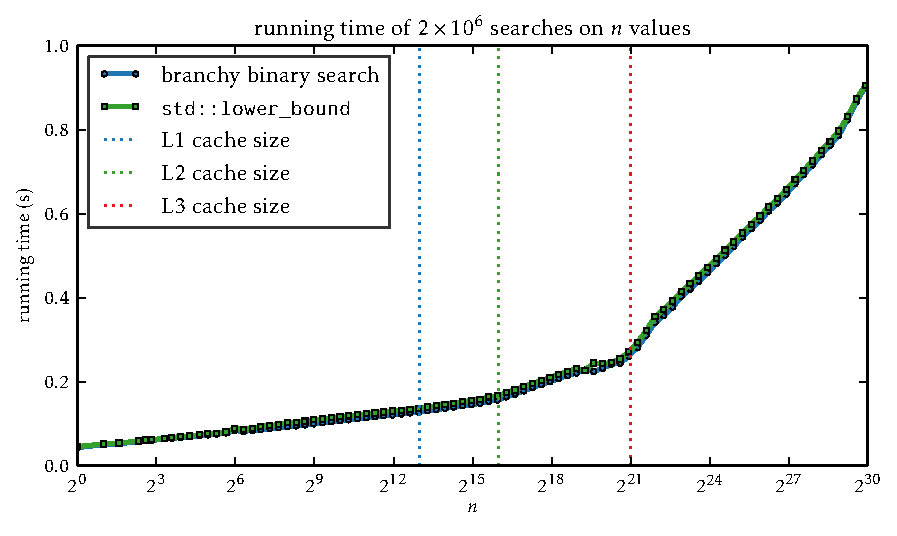
\includegraphics{figs/sorted-i}}
   \caption{The running time of \naive\ binary search and 
            \mintinline{c++}{stl::lower_bound()}.}
   \figlabel{sorted-i}
\end{figure}

If we consider only values of $n$ up to $2^{21}$, shown in
\figref{sorted-ii}, we see an additional change in slope at
$n=2^{16}$.  This is the same effect, but at the L2/L3 cache level; the
4790K has a 256KB L2 cache capable of storing $64K=2^{16}$ data items.
Each additional level of binary search beyond that point incurs an
additional L2 cache miss and an access to the L3 cache.

\begin{figure}
   \centering{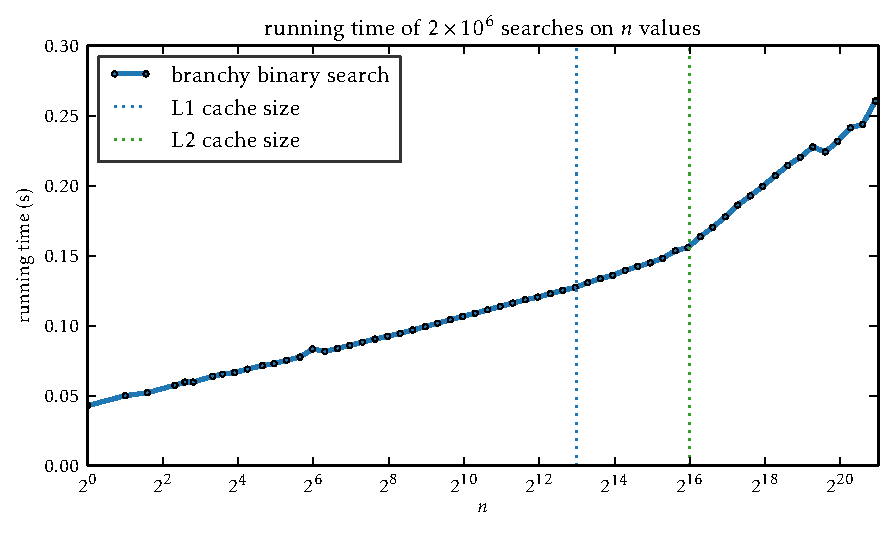
\includegraphics{figs/sorted-ii}}
   \caption{The running time of \naive\ binary search when all data
    fits into L3 cache.}
   \figlabel{sorted-ii}
\end{figure}


\subsubsection{Branch-Free Binary Search}

Readers with experience in micro-optimizing code will see that, for
modern desktop processors, the code in \lstref{nbs} can be optimized
substantially.  There are two problems with this code:

\begin{enumerate}

\item Inside the code is a three-way \mintinline{c++}{if} statement whose
execution path is highly unpredictable. Each of the first two branches
has a close to $50\%$ chance of being executed.  The branch-predictor of
a pipelined processor is forced to guess which of these branches will
occur and load the instructions from this branch into the pipelline.
When it guesses incorrectly (approximately 50\% of the time), the entire
pipeline must be flushed and the instructions for the other branch loaded.

\item The number of iterations of the outer loop is hard to predict. The
loop may terminate early (because \mintinline{c++}{x} was found). Even
when searching for a value \mintinline{c++}{x} that is not present,
unless $n$ has the form $2^k-1$, the exact number of iterations is
different for different values of \mintinline{c++}{x}.  This implies
that the branch predictor will frequently mispredict termination or
non-termination of the loop, incurring the cost of another pipeline flush.

\end{enumerate}

\Lstref{bfbs} shows an alternative implementation of binary search
that attempts to alleviate both problems described above. (This
code implements a variant of Knuth's Algorithm U (Uniform Binary Search)
\cite[Section~6.2.1]{knuth:art}.)  In this implementation, there is no
early termination and, for a given array length \mintinline{c++}{n}, the
number of iterations is fixed (because the value of \mintinline{c++}{n}
always decreases by \mintinline{c++}{half} during each iteration of
the loop).  Therefore, when this method is called repeatedly on the
same array, a good branch-predictor will very quickly learn the number
of iterations of the \mintinline{c++}{while} loop, and it will generate
no further branch mispredictions.

\begin{listing}
\begin{minted}[linenos]{c++}
template<typename T, typename I>
I sorted_array<T,I>::_branchfree_search(T x) const {
    const T *base = a;
    I n = this->n;
    while (n > 1) {
        const I half = n / 2;
        base = (base[half] < x) ? &base[half] : base;
        n -= half;
    }
    return (*base < x) + base - a;
}
\end{minted}
\caption{Source code for branch-free binary search.}
\lstlabel{bfbs}
\end{listing}

In the interior of the \mintinline{c++}{while} loop, there is only one
piece of conditional code, which occurs in Line~7.  For readers unfamiliar
with C's choice operator, this code is equivalent to \mintinline{c++}{if
(base[half] < x) base = &base[half]}, so this line either reassigns
the value of \mintinline{c++}{base} (if \mintinline{c++}{base[half]
< x}) or leaves it unchanged.  The compiler implements this using a
\emph{conditional move} (\mintinline{nasm}{cmov}) instruction so that
there is no branching within the while loop.  For this reason, we call
this \emph{branch-free binary search}.

The use of conditional move instructions to replace branching is a
topic of heated debate (see, e.g., \cite{torvalds:cmov}).  Conditional
move instructions tend to use more clock cycles than traditional
instructions and, in many cases, branch predictors can achieve prediction
accuracies exceeding 95\%, which makes it faster to use a conditional
jump.  In this particular instance, however, the branch predictor will
be unable to make predictions with accuracy exceeding 50\%, making a
conditional move the best choice.  The resulting assembly code, shown in
\lstref{bfbs-asm} is very lean.  The body of the \mintinline{c++}{while}
loop is implemented by Lines~8--15 with the conditional move at Line~12.


\begin{listing}
\begin{minted}[linenos]{nasm}
  .cfi_startproc
  movq    8(%rdi), %rdx       ; move n into rdx
  movq    (%rdi), %r8         ; move a into r8
  cmpq    $1, %rdx            ; compare n and 1
  movq    %r8, %rax           ; move base into rax
  jbe    .L2                  ; quit if n <= 1
.L3:
  movq    %rdx, %rcx          ; put n into rcx
  shrq    %rcx                ; rcx = half = n/2
  leaq    (%rax,%rcx,4), %rdi ; load &base[half] into rdi
  cmpl    %esi, (%rdi)        ; compare x and base[half]
  cmovb   %rdi, %rax          ; set base = &base[half] if x > base[half]
  subq    %rcx, %rdx          ; n = n - half
  cmpq    $1, %rdx            ; compare n and 1
  ja    .L3                   ; keep going if n > 1
.L2:
  cmpl    %esi, (%rax)        ; compare x to *base
  sbbq    %rdx, %rdx          ; set dx to 00..00 or 11...11
  andl    $4, %edx            ; set dx to 0 or 4 
  addq    %rdx, %rax          ; add dx to base
  subq    %r8, %rax           ; compute base - a (* 4)
  sarq    $2, %rax            ; (divide by 4)
  ret
  .cfi_endproc
\end{minted}
\caption{Compiler-generated assembly code for branch-free binary search.}
\lstlabel{bfbs-asm}
\end{listing}

\Figref{sorted-iii} compares the performance of the \naive\ and
branch-free implementations of binary search for array sizes 
ranging from 1 to $2^{16}$.  As expected, the branch-free code is much
faster. After accounting for the overhead of the testing harness, the
branch-free search is approximately twice as fast for $n=2^{16}$.

\begin{figure}
   \centering{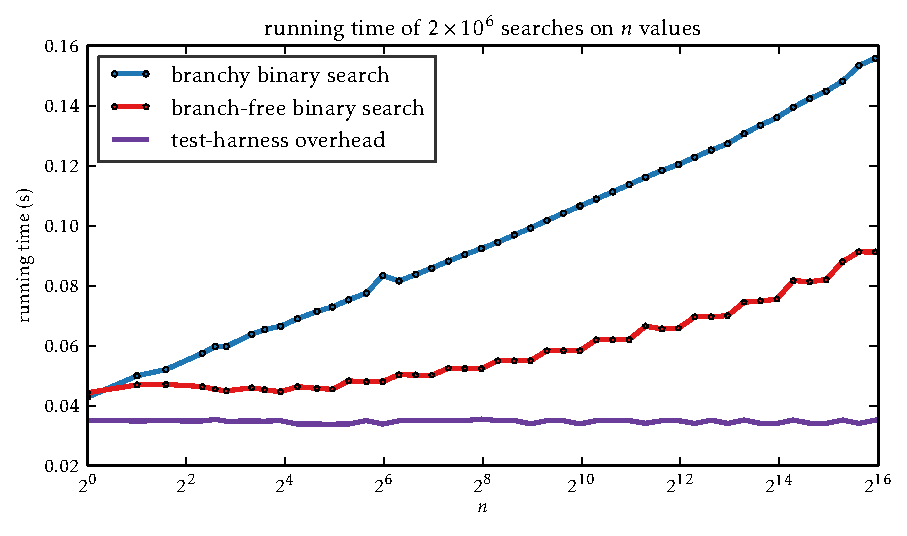
\includegraphics{figs/sorted-iii}}
   \caption{The running times of \naive\ binary search versus
    branch-free binary search when all data
    fits into L2 cache.}
   \figlabel{sorted-iii}
\end{figure}

However, for larger values of $n$ (shown in \figref{sorted-iv}) the
situation changes.  For $n>2^{16}$, the gap begins to narrow slowly
until $n>2^{21}$, at which point it narrows more quickly.  By the time
time $n$ exceeds $2^{22}$, the branch-free code is slower and the gap
between the two continues to widen from this point onward.

\begin{figure}
   \centering{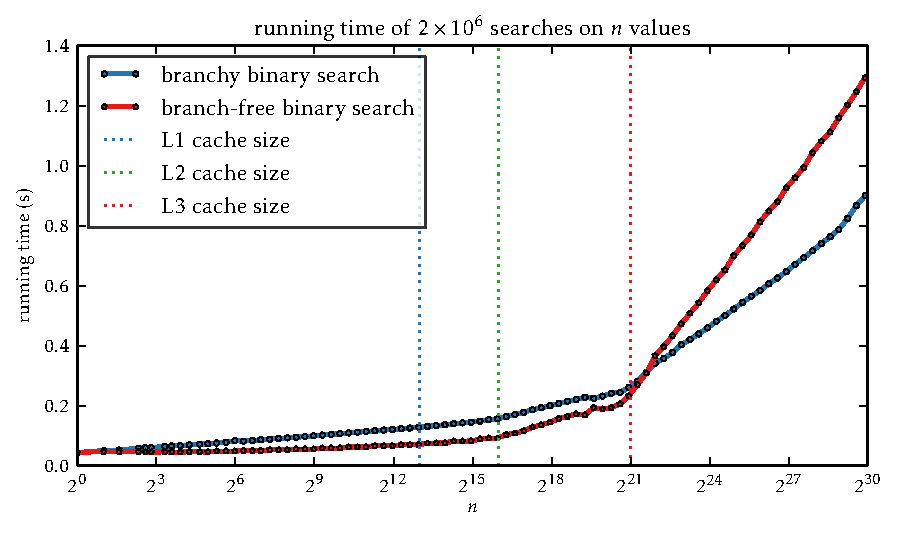
\includegraphics{figs/sorted-iv}}
   \caption{The running times of \naive\ binary search versus
    branch-free binary search for large values of $n$.}
   \figlabel{sorted-iv}
\end{figure}

\subsubsection{Branchy Code, Speculative Execution, and Implicit Prefetching}
\seclabel{sorted-discussion}

The reason for the change in relative performance between branchy
and branch-free binary search was not immediately obvious to us.
After some experimentation, we discovered it comes from the interplay
between branch prediction and the memory subsystem.  In the \naive\
code, the branch-predictor makes a guess at which branch will be taken
and is correct approximately half the time. An incorrrect guess causes a
costly pipeline flush.  However, a correct guess results in the memory
subsystem starting to load the array location needed during the next
iteration of the \mintinline{c++}{while} loop.

For $n<2^{16}$, the entire array fits into L2 cache, and the costs
of pipeline flushes exceed any savings obtained by correct guesses.
However, for larger $n$, each correct guess by the branch-predictor
triggers an L2 (in the range $2^{16}<n<2^{21}$) or an L3 (for $n>2^{21}$)
cache miss sooner than it would otherwise.  The costs of these cache
misses are greater than the costs of the pipeline flushes, so eventually,
the branch-free code loses out to the branchy code.

Since this was not our initial explanation, and since it was not obvious
from the beginning, we gathered several pieces of evidence to support
or disprove this hypothesis.

\begin{enumerate}
\item Assembly-level profiling showed that, for large $n$, the
  branch-free code spends the vast majority of its time loading from
  memory (Line~11, of \lstref{bfbs-asm}).  This is because the register,
  \mintinline{nasm}{rdi},  containing the memory address to load is the
  target of a conditional move (Line~12).  This conditional move has not
  completed because it is still waiting on the results of the previous
  comparison, so execution stalls at this point.

\item Another possible explanation for our results is that the hardware
   prefetcher is, for some reason, better able to handle the branchy
   code than the branch-free code.  This seems unlikely, since the memory
   access patterns for both version are quite similar, and probably too
   complicated for a hardware prefetcher to predict. Nevertheless, we
   ruled out this possibility by disabling the hardware prefetcher and
   running the tests again.\footnote{Prefetching was disabled using the
   \mintinline{console}{wrmsr} utility with register number 0x1a4 and
   value 0xf.  This disables all prefetching \cite{intel:optimizing}.}
   The running-times of the code were unchanged by disabling prefetching.

\item We implemented a version of the branch-free code that adds explicit
   prefetching. At the top of the while loop, it
   prefetches array locations \mintinline{c++}{a[half/2]}
   and \mintinline{c++}{a[half+half/2]} using \texttt{gcc}'s
   \mintinline{c++}{__builtin_prefetch()} builtin, which translates into
   the x86 \mintinline{nasm}{prefetch0} instruction.  The performance of
   the resulting code, shown in \figref{sorted-v} is consistent with our
   hypothesis.  The code is nearly as fast as the branch-free code for
   small values of $n$, but tracks (and even improves) the performance
   of the branchy code for larger values of $n$.

\begin{figure}
   \centering{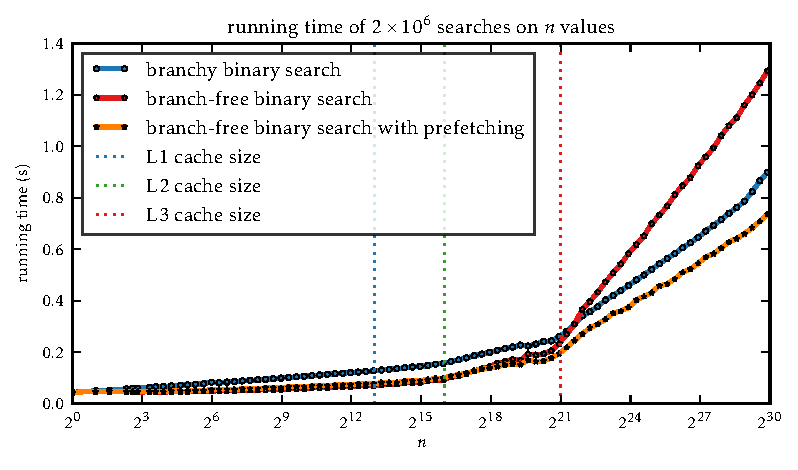
\includegraphics{figs/sorted-v}}
   \caption{Branch-free binary search with explicit prefetching is competitive
    for small values of $n$ and a clear winner for large values of $n$.}
   \figlabel{sorted-v}
\end{figure}

   Note that this code actually causes the memory subsystem to do more
   work, and consumes more memory bandwidth since, in general it loads
   two cache lines when only one will be used.  Nevertheless it is faster
   because the memory bandwidth is more than twice the cache line width
   divided by the memory latency.

\item We ran our code on an Atom 330 processor that we had available. This
   low-power processor was designed to minimize watts-per-instruction
   so it does not do any form of speculative execution, including
   branch prediction. The results, which are shown in \figref{sorted-atom},
   are consistent with our hypothesis.  The branch-free code is faster
   than the branchy code across the full range of values for $n$.
   This is because, on the Atom 330, branches in the branchy code result
   in pipeline stalls that do not help the memory subsystem predict
   future memory accesses.
\end{enumerate}

\begin{figure}
   \centering{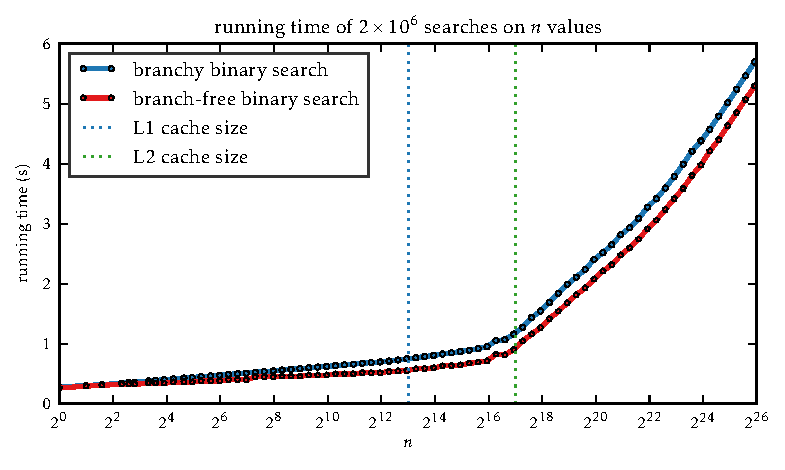
\includegraphics{figs/sorted-atom}}
   \caption{Binary search running-times on the Atom 330. The Atom 330
   has a 512KB L2 cache that can store $2^{17}$ 4-byte integers and does
   not perform speculative execution of any kind.}
   \figlabel{sorted-atom}
\end{figure}

From our study of binary search, we conclude the following lesson about
the (very important) case where one is searching in a sorted array:

\begin{lesson}
  For searching in a sorted array, the fastest method uses branch-free
  code with explicit prefetching.  This is true both on modern pipelined
  processors that use branch prediction and on traditional sequential
  processors.
\end{lesson}

We finish our discussion of binary search by pointing out one lesser-known
caveat:  If $n$ is large and very close to a power of 2, then all
three variants of binary search discussed here will have poor cache
utilization.  This is caused by cache-line aliasing between the elements
at the top levels of the binary search; in a $c$-way associative cache,
these top-level elements are all restricted to use $O(c)$ cache lines.
This problem is observed in the experimental results of Brodal \etal\
\cite[Section~4.2]{brodal.fagerberg.ea:cache} and examined in detail
by the first author \cite{khuong:binary}, who also suggests efficient
workarounds.

\subsection{Eytzinger}

Recall that, in the Eytzinger layout, the data is viewed as being
stored in a complete binary search tree and the values of the nodes in
this virtual tree are placed in the array in the order they would be
encountered in a left-to-right breadth-first traversal.  A nice property
of this layout is that it is easy to follow a root-to-leaf path in the
virtual tree: The value of the root of the virtual tree is stored at
index 0, and the values of left and right children of the node stored
at index $i$ are stored at indices $2i+1$ and $2i+2$, respectively.


\subsubsection{Cache-Use Analysis}
\seclabel{eytzinger-cache-use}

With respect to caching, the performance of searches in an Eytzinger
array should be comparable to that of binary searching in a sorted array,
but for slightly different reasons.

When performing repeated random searches, the top levels of the (virtual)
binary tree are accessed most frequently, with a node at depth $d$
being accessed with probability roughly $1/2^d$.  Since nodes of the
virtual tree are mapped into the array in breadth-first order, the
top levels appear consecutively at the beginning of the array. Thus,
we expect the cache to store, roughly, the first $C$ elements of the
array, which correspond to the top $\log C$ levels of the virtual tree.
As the search proceeds through the top $\log C$ levels, it hits cached
values, but after $\log C$ levels, each subsequent comparison causes
a cache miss.  This results in a total of roughly $\log n-\log C$ cache
misses, just as in binary search.



\subsubsection{Branchy Eytzinger Search}

A branchy implementation of search in an Eytzinger array, shown in
\lstref{eytzinger-i}, is nearly as simple as that of binary search, with
only one slight complication. When branchy binary search completes, the
variable \mintinline{c++}{hi} stores the return value. In Eytzinger search,
we must decode the return value from the value of \mintinline{c++}{i}
at the termination of the \mintinline{c++}{while} loop.  Since we haven't seen
this particular bit-manipulation trick before, we explain it here.


\begin{listing}
\begin{minted}[linenos]{c++}
template<typename T, typename I>
I eytzinger_array<T,I>::branchy_search(T x) const {
    I i = 0;
    while (i < n) {
        if (x < a[i]) {
            i = 2*i + 1;
        } else if (x > a[i]) {
            i = 2*i + 2;
        } else {
            return i;
        }
    }
    I j = (i+1) >> __builtin_ffs(~(i+1));
    return (j == 0) ? n : j-1;
}
\end{minted}
\caption{Branchy implementation of search in an Eytzinger array.}
\lstlabel{eytzinger-i}
\end{listing}

In the Eytzinger layout, the $2^d$ nodes of the virtual tree at depth $d$
appear consecutively, in left-to-right order, starting at index
$\sum_{k=0}^{d-1}2^k = 2^d-1$.  Therefore, an array position
$i\in\{2^d-1,\ldots,2^{d+1}-2\}$ corresponds to a node, $u$, of the
virtual tree at depth $d$. Furthermore, the binary representation,
$b_w,b_{w-1},\ldots,b_0$, of $i+1$ has a nice interpretation:

\begin{itemize}
  \item The bits $b_w=b_{w-1}=\cdots=b_{d+1}=0$, since $i+1 < 2^{d+1}$.
  \item The bit $b_d=1$ since $i+1\ge 2^d$.
  \item The bits $b_{d-1},\ldots,b_{0}$ encode the path,
    $u_1,\ldots,u_{d}$, from the root of the virtual tree to
    $u=u_{d}$: For each $k\in\{1,\ldots,d-1\}$, if $u_{k+1}$ is the left
    (respectively, right) child of $u_k$, then $b_{d-k}=0$ (respectively,
    $b_{d-k}=1$).
\end{itemize}

Therefore, the position of the highest order 1-bit of $i+1$  tells
us the depth, $d$, of the node $u$ and the bits $b_{d-1},\ldots,b_{0}$ tell
us the path to $u$.  This is true even if $i\ge n$, in which case we
can think of $u$ as an external node of the virtual tree (that stores
no data).  To answer a query, we are interested in the last node,
$w$, on the path to $u$ at which the path proceeded to a left child.
This corresponds to the position, $r$, of the lowest order 0 bit in the
binary representation of $i+1$.  Furthermore, by right-shifting $i+1$
by $r+1$ positions we obtain an integer $j$ such that:

\begin{enumerate}
  \item $j-1$ is the index of $w$ in the array (if $w$ exists), or
  \item $j=0$ if $w$ does not exist (because the path to $u$ never proceeds 
        from a node to its left child).
\end{enumerate}

The latter case occurs precisely when we search for a value
\mintinline{c++}{x} that is larger than any value in the array. The
last two lines of code in \lstref{eytzinger-i} extract the value of $j$
from the value of $i$ and convert this back into a correct return value.
The only non-standard instruction used here is \mintinline{console}{gcc}'s
\mintinline{c++}{__builtin_ffs} builtin that returns one plus the index
of the least significant one bit of its argument.  This operation,
or equivalent operations, are supported by most hardware and C/C++
compilers \cite{wiki:find}.

\subsubsection{Branch-Free Eytzinger Search}

A branch-free implementation of search in an Eytzinger array---shown
in \lstref{eytzinger-ii}---is also quite simple. Unfortunately, unlike
branch-free binary search, the branch-free Eytzinger search is unable
to avoid variations in the number of iterations of the while loop,
since this depends on the depth (in the virtual tree) of the leaf that
is reached when searching for \mintinline{c++}{x}.  When $n=2^h-1$ for
some integer $k$, then all leaves have the same depth but, in general,
there will be leaves of depths $h$ and depth $h-1$, where $h=\lceil\log
(n+1)\rceil-1$ is the height of the virtual tree.

\begin{listing}
\begin{minted}[linenos]{c++}
template<typename T, typename I>
I eytzinger_array<T,I>::branchfree_search(T x) const {
    I i = 0;
    while (i < n) {
        i = (x <= a[i]) ? (2*i + 1) : (2*i + 2);
    }
    I j = (i+1) >> __builtin_ffs(~(i+1));
    return (j == 0) ? n : j-1;
}
\end{minted}
\caption{Branch-free implementation of search in an Eytzinger array.}
\lstlabel{eytzinger-ii}
\end{listing}

The performance of the branchy and branch-free versions of search
in an Eytzinger array is shown in \figref{eytzinger-i}.  Branch-free
Eytzinger search very closely matches the performance of branch-free
binary search. As expected, there is an increase in slope at $n=2^{16}$
and $n=2^{21}$ since these are the number of 4-byte integers that can
be stored int the L2 and L3 caches, respectively.

However, the performance of the branchy Eytzinger implementation is
much better than expected for large values of $n$. Indeed, it is much
faster than the branchy implementation of binary search, and even
faster than our fastest implementation of binary search.

\begin{figure}
   \centering{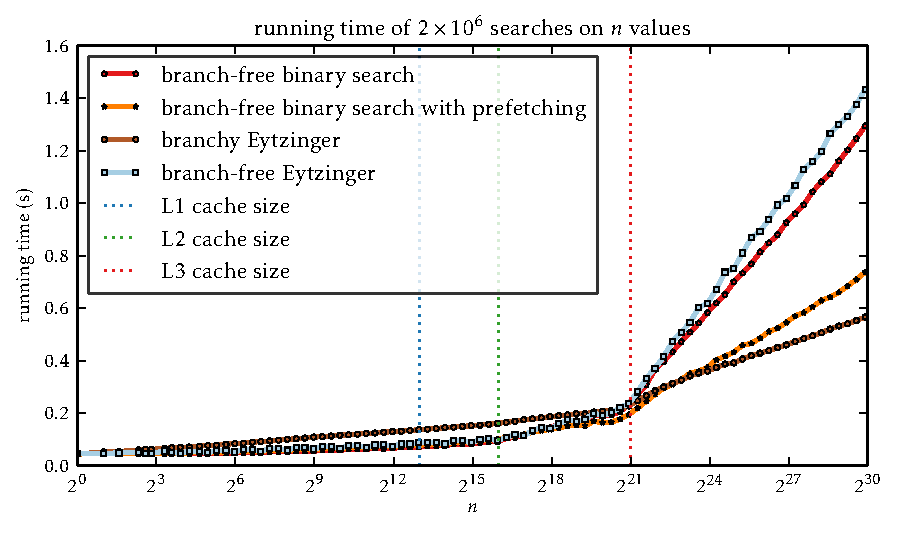
\includegraphics{figs/eytzinger-i}}
   \caption{The performance of branchy and branch-free Eytzinger search.}
   \figlabel{eytzinger-i}
\end{figure}

\subsubsection{Why Eytzinger is so Fast}

Like branchy binary search, the branchy implementation of search in
Eytzinger array is so much faster than expected because of the interaction
between branch prediction and the memory subsystem.  However, in the
case of the Eytzinger layout, this interaction is much more efficient.

To understand why the branchy Eytzinger code is so fast recall that,
in the Eytzinger layout, the nodes are laid out in breadth-first
search order,  so the two children of a node occupy consecutive array
locations $2i$ and $2i+1$. More generally, for a virtual node, $u$,
that is assigned index $i$, $u$'s $2^\ell$ descendants at distance
$\ell$ from $u$ are consecutive and occupy array indices $2^\ell i +
2^{\ell}-1,\ldots,2^{\ell} i + 2^{\ell+1}-1$.

In our working example of 4-byte data with 64-byte cache lines, the
sixteen great-great grandchildren of the virtual node stored at position
$i$ are stored at array locations $16i+15,\ldots,16i+30$.  Assuming that
the first element of the array is the first element of a cache line,
this means that, of those 16 descendants, 15 are contained in a single
cache line (the ones stored at array indices $16i+16,\ldots,16i+30$.)

With the Intel 4790K's 20--24 cycle pipeline, instructions in
the pipeline can be several iterations ahead in the execution of the
\mintinline{c++}{while} loop, which only executes 5--6 instructions per
iteration.  The probability that the branch-predictor correctly guesses
the execution path of four consecutive iterations is only about 1/16,
and a flush of (some of) the pipeline is likely.  However, even if the
branch predictor does not guess the correct execution path, it most likely
(with probability 15/16) guesses an execution path that loads the correct
cache line.  Even though the branch predictor loads instructions that will
likely never be executed, their presence in the pipeline causes the memory
subystem to begin loading the cache line that will eventually be needed.

Knowing this, there are two optimizations we can make:
\begin{enumerate}
  \item We can add an explicit prefetch instruction to the branch-free code
    so that it loads the correct cache line.  The resulting code is shown
    in \lstref{eytzinger-iii}.

  \item We can align the array so that \mintinline{c++}{a[0]} is the
    second element of a cache line.  In this way, all 16 great-great
    grandchildren of a node will always be stored in a single cache line.
\end{enumerate}

\begin{listing}
\begin{minted}[linenos]{c++}
template<typename T, typename I>
I eytzinger_array<T,I>::branchfree_search(T x) const {
    I i = 0;
    while (i < n) {
        __builtin_prefetch(a+(multiplier*i + offset));
        i = (x <= a[i]) ? (2*i + 1) : (2*i + 2);
    }
    I j = (i+1) >> __builtin_ffs(~(i+1));
    return (j == 0) ? n : j-1;
}
\end{minted}
\caption{Branch-free prefetching implementation of search in an
         Eytzinger array. (The value of \mintinline{c++}{multiplier}
         in this code is the cache line width, $B$, and the value of
         \mintinline{c++}{offset} is $\lfloor3B/2\rfloor-1$.)}
\lstlabel{eytzinger-iii}
\end{listing}

The results of implementing both of these optimizations are shown
in \figref{eytzinger-ii}.\footnote{Although \figref{eytzinger-ii}
shows the results of implementing both these optimizations, we did test them
individually. Realigning the array gives in only a small improvement in
performance; the real improvements come from combining branch-free code and
explicit prefetching.}  With these optimizations, the change in slope
at the L2 cache limit disappears; four iterations of the search loop is
enough time to prefetch data from the L3 cache.  Once the L3 cache limit
is reached, the behaviour becomes similar to the branchy implementation,
but remains noticeably faster, since the branch-free code does not cause
pipeline flushes and always prefetches the correct cache line 4 levels
in advance.

\begin{figure}
   \centering{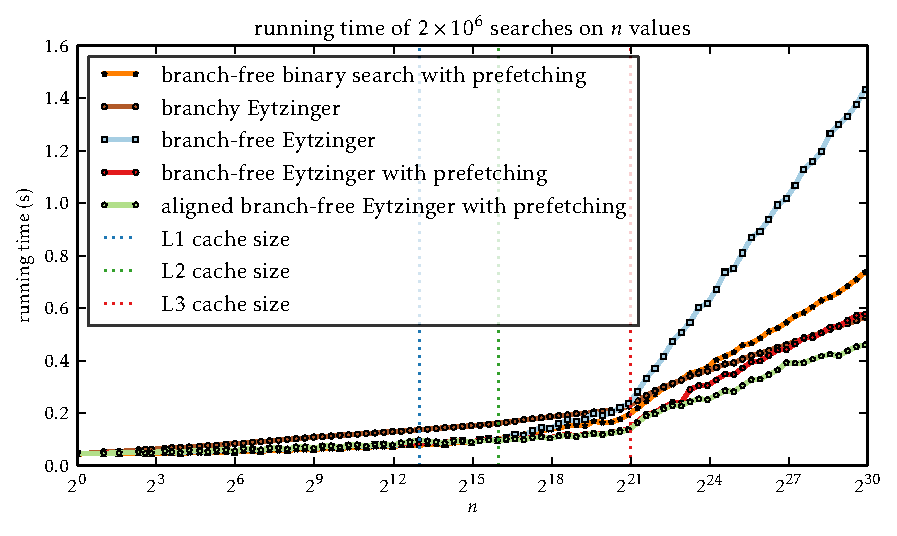
\includegraphics{figs/eytzinger-ii}}
   \caption{The performance of branch-free Eytzinger with prefetching.}
   \figlabel{eytzinger-ii}
\end{figure}

\figref{eytzinger-iii} compares Eytzinger search with binary search for
small values of $n$ ($n\le 2^{16}$).  At this scale
the branch-free Eytzinger code is very close, but not quite as fast
as the best binary search implementations.  Something else evident in
\figref{eytzinger-ii} is a ``bumpiness'' of the Eytzinger running-times
as a function of $n$.  This bumpiness is caused by branch mispredictions
during the execution of the while loop.  The search times are especially
low when $n$ is close to a power of two because in this case nearly all
searches perform the same number of iterations of the while loop (since
the underlying tree is a complete binary tree of height $h$ with nearly
all leaves at same level $h$).  The branch predictor quickly learns
the value of $h$ then correctly predicts the final iteration.  On the
other hand, when $n$ is far from a power of 2, the number of iterations
is either $h$ or $h-1$, each with non-negligible probability, and the
branch predictor is unable to accurately predict the final iteration of
the while loop.

\begin{figure}
   \centering{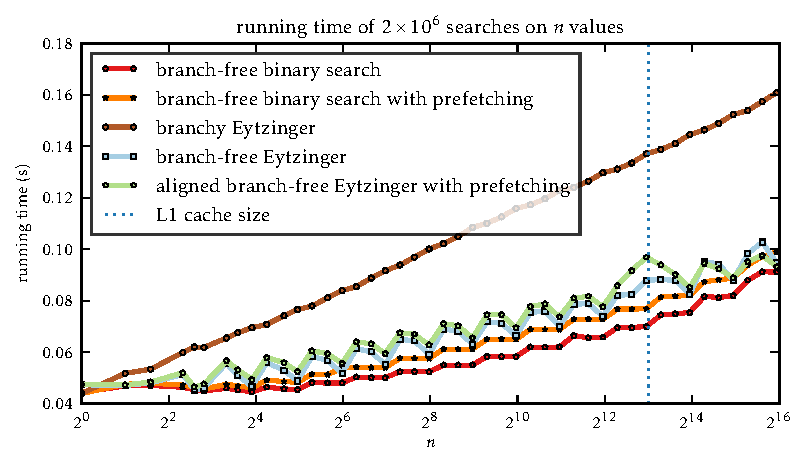
\includegraphics{figs/eytzinger-iii}}
   \caption{Eytzinger versus binary search for small values of $n$.}
   \figlabel{eytzinger-iii}
\end{figure}



\begin{lesson}
  For the Eytzinger layout, branch-free search with explicit prefetching
  is the fastest search implementation. For small values of $n$,
  this implementation is competitive with the fastest binary search
  implementations. For large values of $n$, this implementation
  outperforms all versions of binary search by a wide margin.
\end{lesson}

\subsubsection{A Mixed Eytzinger/Sorted Layout}

We conclude this section with a discussion of a mixed layout suggested by
the cache-use analyses of binary and Eytzinger search.  Conceptually, this
layout implements a binary search tree (laid out as an Eytzinger array)
whose leaves each contain blocks of $B$ values (stored in sorted order).

More specifically, the first part of the array contains values $x_0,\ldots
x_{2^{h}-2}$ stored using the Eytzinger layout and the second part of
the array contains values $y_0,\ldots,y_{n-2^h}$ in sorted order.  Here,
the value of $h$ is the minimum integer such that $2^{h}-1 + B2^h \ge n$
and the values in the first part of the array are chosen so that
\[
    y_0<\cdots<y_{B-1} < x_0 < y_{B}<\cdots<y_{2B-1} < x_1 < \cdots
\]
In this way, a search in the first part of the array usually narrows
down the answer to a block of $B$ consecutive values in the second part
of the array, and these values are stored in a single cache line. Using
this layout, one can store up to $BC$ values and a search will incur
only a single cache miss. (The Eytzinger layout lives entirely in the
cache of size $C$ and reduces the problem to a binary search in a single
cache line of size $B$.)

Both the search in the Eytzinger array and the sorted block can be
implemented using fast branch-free code so, in theory, this layout
should be faster than either the Eytzinger or the sorted layout.
This is true: In \figref{mixed-i} we see that this code effectively
increases the cache size when compared to the branch-free Eytzinger code.
Though there is an increase in slope at $n=2^{21}$, it does not become
as severe as the Eytzinger code until $n=2^{25}$.  (In \figref{mixed-i}
both implementations are branch-free and neither use prefetching.)

\begin{figure}
   \begin{center}
     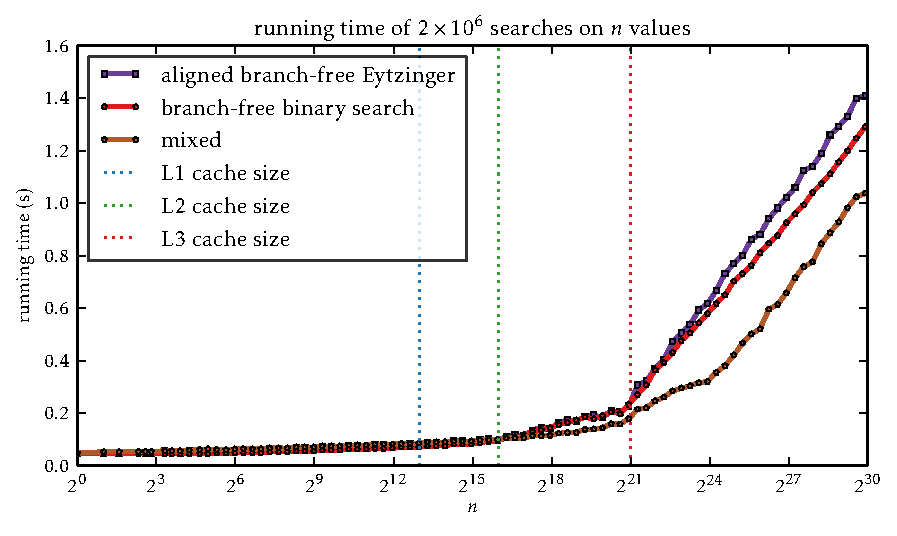
\includegraphics{figs/mixed-i}
   \end{center}
   \caption{Performance of the branch-free mixed layout (without prefetching).}
   \figlabel{mixed-i}
\end{figure}

However, this mixed layout is unable to beat branch-free Eytzinger
search with explicit prefetching. This is true even when the mixed
layout uses prefetching in the Eytzinger part of its search (which has
the side-effect of prefetching the correct block for the second part
of the search). \Figref{mixed-ii} compares branch-free Eytzinger with
prefetching and a prefetching version of the mixed layout.  The two
layouts are virtually indistinguishable with respect to performance.

\begin{figure}
   \begin{center}
     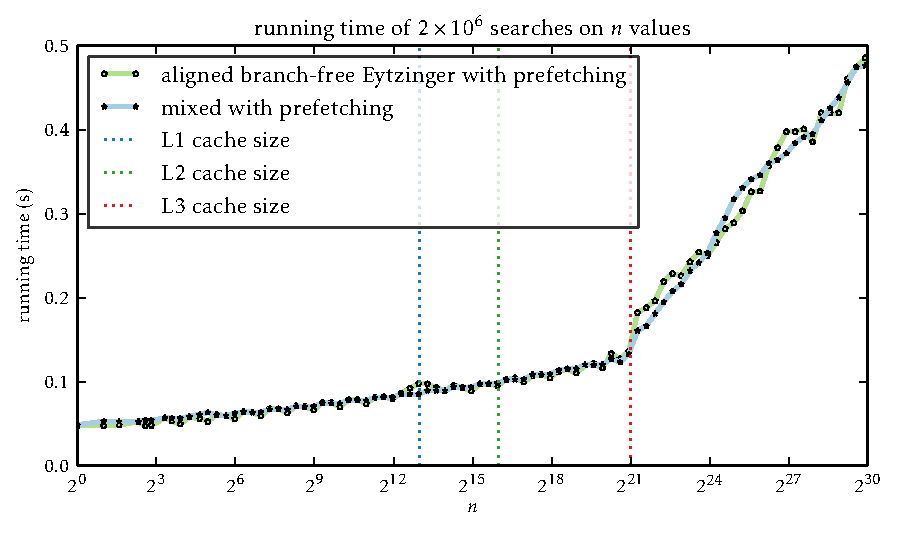
\includegraphics{figs/mixed-ii}
   \end{center}
   \caption{Performance of the branch-free mixed layout with prefetching.}
   \figlabel{mixed-ii}
\end{figure}

\begin{lesson}
  Although the mixed layout looks promising, it is unable to beat
  the performance of branch-free Eytzinger with prefetching and is
  considerably more complicated to implement.
\end{lesson}

\subsection{Btree}

Recall that the $(B+1)$-tree layout simulates search on a $(B+1)$-ary
search tree, in which each node stores $B$ values.  The nodes of this
$(B+1)$-ary tree are laid out in the order they are encountered in
a breadth-first search.  The Eytzinger layout is a special
case of the Btree layout in which $B=1$. As with the Eytzinger layout, there
are formulas to find the children of a node: For $j\in\{0,\ldots,B\}$, the
$j$-th child of the node stored at indices $i,\ldots,i+B-1$ is stored
at indices $f(i,j),\ldots,f(i,j)+B-1$ where $f(i,j)=i(B+1)+(j+1)B$.

The code for search in a $(B+1)$-tree layout consists of a while loop
that contains an inner binary search on a subarray (block) of length
$B$. Very occasionally, the Btree search completes with one binary search
on a block of size less than $B$. The block size, $B$, is chosen to fit
neatly into one cache line. On our test machines, cache lines are 64
bytes wide, so we chose $B=16$ for 4-byte data. Preliminary testing with
other block sizes showed that this theoretically optimal choice for $B$
is also optimal in practice.

\subsubsection{Cache-Use Analysis}

The height of a $(B+1)$ tree that stores $n$ keys is approximately
$\log_{(B+1)} n$.  A search in a $(B+1)$-tree visits $\log_{(B+1)} n$
nodes, each of which is contained in a single cache line, so a search
requires loading only $\log_{(B+1)} n$ cache lines.

By the same reasoning as before, we expect that the top $\log_{(B+1)} C$
levels of the $(B+1)$-tree, which correspond to the first $C$ elements
of the array, will be stored in the cache.  Thus, the number of cache
misses that occur when searching in a $(B+1)$-tree is
\[
    \log_{(B+1)}n - \log_{(B+1)} C 
         = \frac{\log n - \log C}{\log (B+1)} \enspace .
\]
Observe that this is roughly a factor of $\log(B+1)$ fewer cache misses
than the $\log n-\log C$ cache misses incurred by binary search or
Eytzinger search.

In our test setup, with $B=16$, we therefore expect that the number
of cache misses should be reduced by a factor of $\log 17\approx
4.09$. When plotted, there should still be an increase in slope that
occurs at $n=2^{21}$, but it should be significantly less pronounced
than in binary search.

\subsubsection{Na\"{\i}ve and Branch-Free Btree Implementations}

We made and tested several implementations of the Btree search algorithm,
including a completely na\"{\i}ve implementation, an implementation that
uses C++ templates to unroll the inner search, and an implementation
that uses C++ templates to generate an unrolled branch-free inner search.

\Figref{btree-i} shows the results for our three implementations of
Btree search as well as branch-free binary search and our best implementation
of Eytzinger search.  For small values of $n$, the na\"ive implementation
of Btree search is much slower than the unrolled implementations, and there
is little difference between the two unrolled implementations. For values
of $n$ larger than the L3 cache, the running time of all three Btree
search implementations becomes almost indistinguishable. This is expected
since, for large $n$, the running-time becomes dominated by L3 cache
misses, which are the same for all three implementations.

\begin{figure}
   \centering{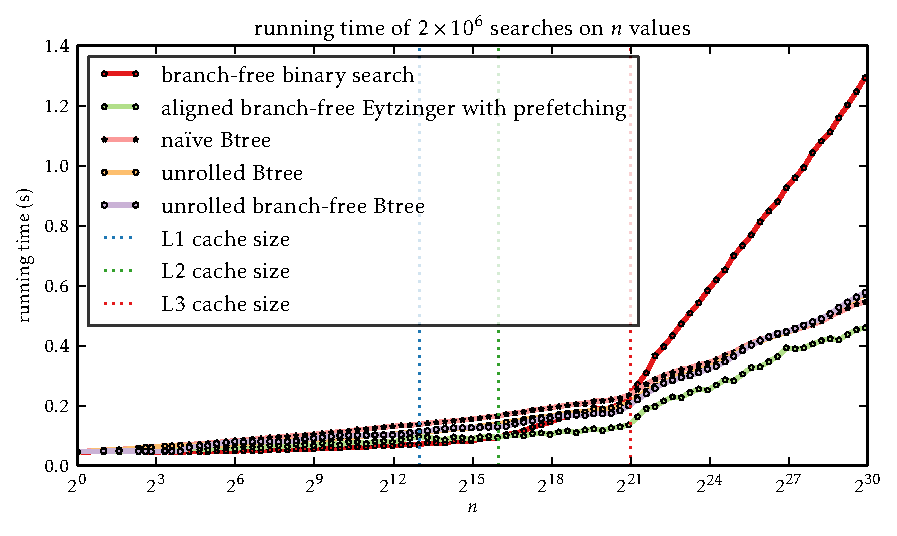
\includegraphics{figs/btree-i}}
   \caption{The performance of Btrees search algorithms.}
   \figlabel{btree-i}
\end{figure}


Compared to branch-free binary search, the Btree search implementations
behave as the cache-use analysis predicts:  Both algorithms are fast for
$n<2^{21}$ after which both show an increase in slope. At this point,
the the slope for branch-free binary search is approximately 3.8 times
larger than that of the Btree search. (The analysis predicts a factor
of $\log 17\approx 4.09$.)

All three implementations of Btree search perform worse than our best
Eytzinger search implementation across the entire spectrum of values
of $n$.  For small values of $n$, this is due to the fact that Eytzinger
search is a simpler algorithm with smaller constants.  One reason
Eytzinger search has smaller constants is that the inner binary search
of Btrees is inherently inefficient. Our virtual Btree stores 16 keys per
node, so the inner binary search has 17 possible outcomes, and therefore
requires $\lceil\log_2 17\rceil=5$ comparisons in some cases (and in
all cases for the branch-free code).  This could fixed by using 16-ary
trees instead, but then the number of keys stored in a block would be 15,
which does not align with cache lines.  We tested 16-ary trees and found
them to be slower than 17-ary trees for all values of $n$.\footnote{A
third alternative is to store 15 keys in blocks of size 16, but this would
be outside the model we consider, in which all data resides in a single
array of length $n$.}

For values of $n$ larger than the L3 cache size, Eytzinger search and
Btree search have the same rate of growth, but Eytzinger search starts
out being faster and remains so.  That the two algorithms have the same
rate of growth is no coincidence: This growth is caused by RAM latency.
In the case of Btrees, the time between finishing the search in one
node and beginning the search in the next node is lower-bounded by the
time needed to fetch the next node from RAM.  In the case of Eytzinger
search, the time it takes to advance from level $\ell$ in the implicit
search tree to level $\ell+4$ is lower-bounded by the time needed to fetch
the node at level $\ell+4$ from RAM.  Thus, both algorithms pay one unit of
latency for every 4 or 5 comparisons.

\Figref{btree-ii} compares Btrees with Eytzinger search for values
of $n$ smaller than the L3 cache size.  One interesting aspect of
this plot is that the Btree plots have a slight increase in slope
at $n=2^{16}$---at the point in which the data exceeds the L2 cache
size---while the Eytzinger search algorithm shows almost no change in
behaviour.  This is because Btree search work synchronously with the memory
subsystem; each Btree node is searched using 4--5 comparisons and
then the memory subsystem begins loading the next node (from L3 cache).
The Eytzinger search on the other hand begins loading the node at level
$\ell+4$ and continues to perform comparisons at levels $\ell$, $\ell+1$,
$\ell+2$, and $\ell+3$ while the memory subsystem asynchronously fetches
the node at level $\ell+4$. This effectively hides the L3 cache latency.

\begin{figure}
   \centering{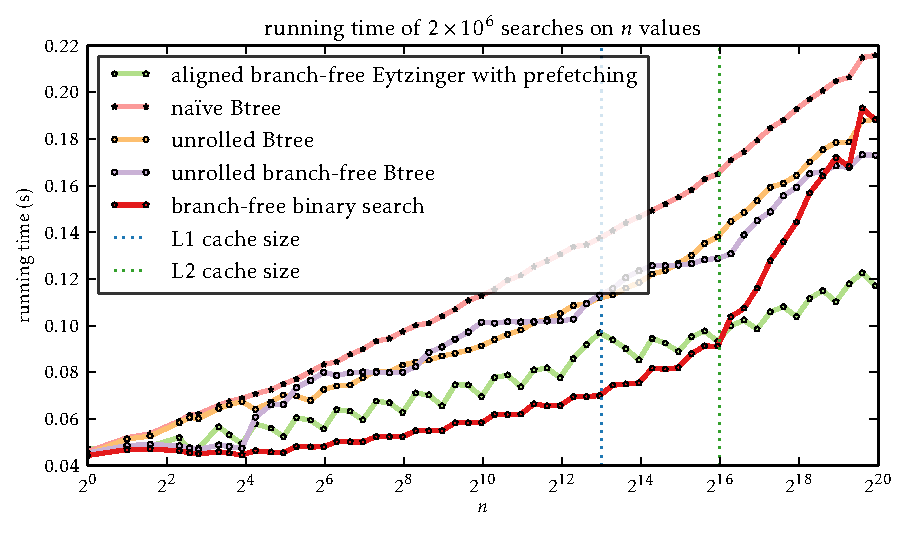
\includegraphics{figs/btree-ii}}
   \caption{The performance of Btree search for small values of $n$.}
   \figlabel{btree-ii}
\end{figure}

\begin{lesson}
  Even though it moves $B$ times more data between levels of the cache
  hierarchy, Eytzinger search with explicit prefetching outperforms
  Btrees.  It does this by exploiting parallelism within the memory
  subsystem and between the processor and memory subsystem.
\end{lesson}

%17-trees, which are theoretically the most promising, unfortunately lose
%out simply because the constants they incur are too large.  
%Unlike the Eytzinger layout, the Btree layout is unable to take much
%advantage of implicit or explicit prefetching.  
%
%In summary, $(B+1)$-trees must make a choice between being efficient in
%terms of the number of comparisons or being efficient in terms of the
%the number of cache misses.  In external memory applications where cache
%misses are orders of magnitude slower than comparisons, this is an easy
%choice. For internal memory, unfortunately, there is no good choice:
%both are slower than a fast Eytzinger implementation.
%
%In external memory applications---for which B-trees were originally designed---it is clear
%
%
%The performance
%We implemented several variations of Btree search:
%
%several variations of Btree searches:
%
%Some also tried:  Btree with Eytzinger layouts.
%
\subsection{Van Emde Boas}

Unlike the Btree layout, the Van Emde Boas layout is parameter free.
It is a recursive layout that provides asympotically optimal behaviour
for any cache line width, $B$.  In the case where there are multiple
levels of cache with different cache line widths, the van Emde Boas
layout is asymptotically optimal for all levels simultaneously.  Indeed,
for any value of $B$, a search in a van Emde Boas layout can be viewed
as searching in a sequence of binary trees whose heights are in the
interval $((1/2)\log B,\log B]$, and each of these subtrees is stored
in a contiguous subarray (and therefore in at most 2 cache lines).
The sum of the heights of these subtrees is $\lceil\log n\rceil$.


\subsubsection{Cache-Use Analysis}

The cache-use analysis of the vEB layout approximates that of B-trees.
We expect to find the most frequently accessed subtrees in the cache,
which correspond, roughly, to the first $\log C$ iterations of the search
algorithm.  Beyond this point, the search passes through a sequence of
subtrees whose height is in the interval $((1/2)\log B,\log B]$ and each of
which is contained in at most two cache lines.  Thus, the number of cache
misses we expect to see is about $O((\log n - \log C)/\log B)$.  Here,
we use big-Oh notation since the exact leading constant is somewhere
between $1$ in the best case and $4$ in the worst case.

\subsubsection{VeB Implementations}

To search in a van Emde Boas layout one needs code that can determine
the indices of the left and right child of each node in the virtual
binary tree.  Unlike, for example, the Eytzinger layout, this is not at
all trivial. We experimented with two approaches to navigating the van
Emde Boas tree: machine bit manipulations and lookup tables.  It very
quickly became apparent that lookup tables are the faster method.

Our implementations store two or three precomputed lookup tables whose
size is equal to the height of the van Emde Boas tree. In addition to
these lookup tables, one must also store the path, \mintinline{c++}{rtl},
from the root to the current node as well as an an encoding,
\mintinline{c++}{p}, of the path from the root to the current node, where
each bit of \mintinline{c++}{p} represents a left turn (0) or a right
turn (1) in this path.  Brodal \etal\ \cite{brodal.fagerberg.ea:cache}
reached the same conclusion when designing their implementation of the
van~Emde~Boas layout.  The most obvious (branchy) code implementing this
algorithm is shown in \lstref{veb}

\begin{listing}
\begin{minted}[linenos]{c++}
template<typename T, typename I>
I veb_array<T,I>::search(T x) {
    I rtl[MAX_H+1];
    I j = n;
    I i = 0;
    I p = 0;
    for (int d = 0; i < n; d++) {
        rtl[d] = i;
        if (x < a[i]) {
            p <<= 1;
            j = i;
        } else if (x > a[i]) {
            p = (p << 1) + 1;
        } else {
            return i;
        }
        i = rtl[d-s[d].h0] + s[d].m0 + (p&s[d].m0)*s[d].m1;
    }
    return j;
}
\end{minted}
\caption{Source code for branchy vEB search.}
\lstlabel{veb}
\end{listing}

In addition to the code in \lstref{veb}, we also implemented (as much as
possible) a branch-free version of the vEB code.  Performance results for
the vEB search implementations are shown in \figref{veb-i}, along with our
best implementations of Btree search and Eytzinger arrays.  As seen with other
layouts, the branch-free implementation is faster until we exceed the size
of the L3 cache, at which point the branchy implementation starts to catch
up. However, in this case, the branchy implementation has a lot of ground
to make up and only beats the branch-free implementation for $n>2^{25}$.

\begin{figure}
   \centering{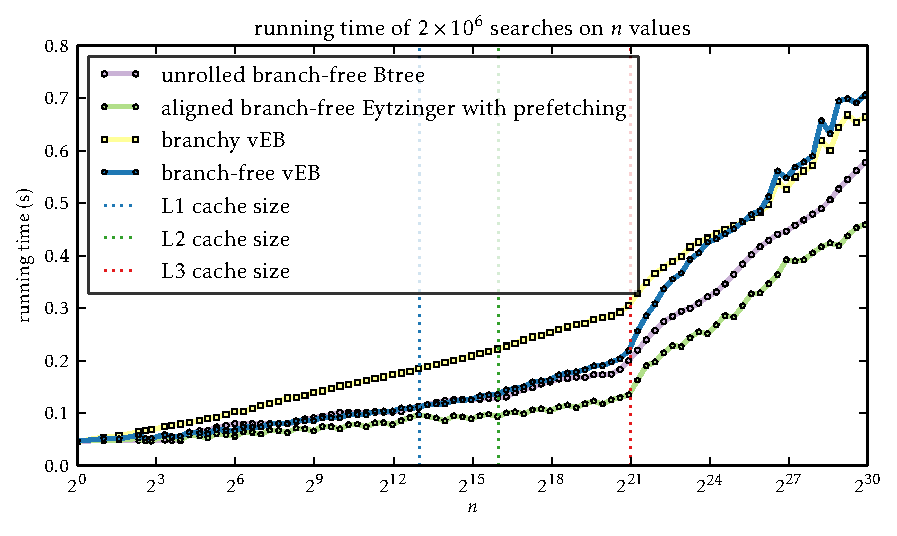
\includegraphics{figs/veb-i}}
   \caption{The performance of the vEB layout.}
   \figlabel{veb-i}
\end{figure}

The branch-free version of the vEB code is competitive with Btrees
until $n$ exceeds the L3 cache size.  At this point, the vEB code becomes
much slower.  This is because the vEB layout only minimizes the number
of L3 cache misses to within a constant factor.  Indeed, the subtrees
of a vEB tree have sizes that are odd and will therefore never be
perfectly aligned with cache boundaries.  Even in the (extremely lucky)
case where a vEB search goes through a sequence of subtrees of size 15,
each of these subtrees is likely to be split across two cache lines,
resulting in twice as many cache misses as a Btree layout.

\begin{lesson}
  The vEB layout is a useful theoretical tool, and may be useful in
  external memory settings, but it is not useful for in-memory searching.
\end{lesson}

%\section{Other Possible Strategies}
%\seclabel{other}
%
%In our experiments, we tried other approaches that seemed promising but that we were unable to make headway on. We outline some of these here:
%
%\subsection{A B-Tree Eytzinger Layout}
%
%We implemented a version of B-trees in which each node was laid out as an
%Eytzinger array.  The idea behind this implementation was to account for
%the fact that loading a cache line is a not an atomic operation. Except
%for the first word requested, the words in a cache line are loaded in
%left-to-right order so the first word is available earlier than, say,
%the fourth word. For example, the DDR-3 RAM in our test machine has a
%first-word latency of approximately 10ns and a fourth-word latency of
%approximately 14ns. Since a search in an Eytzinger accesses the array
%indices in increasing order, the search can start as soon as the first
%word of the cache line is loaded.
%
%A preliminary implementation of this idea did not show any noticeable
%improvement in running time on most of the platforms we tested. A noteable
%exception was the Atom 330, for which the mixed layout was a noticeable
%improvement over the standard B-Tree layout.
%
%\subsection{Blocked Eytzinger Arrays}
%
%The cache-use analysis of the Eytzinger array in
%\secref{eytzinger-cache-use} shows that the number of cache misses during
%a search is roughly $\log n-\log C$. Unlike binary search the $\log C$
%cache hits occur at the beginning of the search, which corresponds to
%searching in the top levels of the virtual tree.  We experimented with
%reducing the number of cache misses to $\log n -\log C - \log B$ by
%treating the first (roughly) $n/(B+1)$ elements of the array as an index
%into (roughly) $n/(B+1)$ blocks each of size $B$. The first part of the
% array was then laid out as an Eytzinger array and the second part was
% stored in sorted order.
%
%A search in this hybrid layout involved a search in the Eytzinger array
%followed by a binary search in a block of size $B$.  Although this hybrid
%layoutdoes reduce the number of cache misses, it does not provide any
%performance improvement over our fastest implementation of search in the
%Eytzinger layout. The reason is that the algorithm pays the full latency
%penalty for the final cache miss, since it can not predict which block
%in the second part of the array is needed until the Eytzinger search in
%the first part of the array is complete.

\section{A Theoretical Model}
\seclabel{model}

There is currently no theoretical model of caches or I/O that predicts
that Eytzinger search is competitive with (and certainly not faster than)
Btrees.  The I/O model \cite{aggarwal.vitter:input} predicts that the
Eytzinger layout is a factor of $\log B$ slower than the Btree layout.
However, we can augment the I/O model so that the cache line width,
measured in data items, is $B$, the latency, measured in time units, for
reading a cache line is $L$, and the bandwidth, measured as the number
of cache lines that can be read per time unit, is $W$.\footnote{The I/O
model already has the parameter $B$, so the only real addition to the
model here is the bandwidth parameter $W$, since we can take $L=1$,
without loss of generality.}  In this model, the time to search in a
Btree is roughly
\[
     (L+c)\log_B n
\]
where $c=O(\log B)$ is the time to search on an (in-memory) block
of size $B$.  This is because a B-tree search consists of $\log_B n$
rounds where each round requires loading a cache line (at a cost of $L$)
and searching that cache line (at a cost of $c$).

On the other hand, if $WL > \log B$, then the memory subsystem can
handle $\log B$ cache line requests in parallel without any additional
overhead. In this case, then the running-time of Eytzinger search with
prefetching is roughly
\[
    \max\{L,c\}\log_B n \enspace .
\]
(Here we assume that the local computation time for $\log B$ levels of
Eytzinger search and the local computation time to do binary
search on a Btree block of size $B$ is the same $c$.)  This analysis
shows that our experimental results do have a theoretical explanation.
It also suggests two possible extensions of our experiments.

\subsection{Deeper Prefetching in Eytzinger Search}

If there is really an excess of bandwidth so that, for example, $WL >
2^t\log B$, then the prefetching for the Eytzinger search can be extended
so, when accessing a virtual node, $v$, in the Eytzinger tree we prefetch
$v$'s $2^tB$ descendants at distance $t+\log B$ from $v$ using $2^t$
prefetch instructions.

We implemented and tested this idea and found that, for the 4-byte data
studied throughout this paper, it did not yield any speedup with $t=1$ and
was significantly slower with $t=2$.  This agrees with our analysis and
the latency/bandwidth characteristics of our machine (\secref{bandwidth}).
On our machine, $WL\approx 4.7$ and, with 4-byte data, $B=16$, so
$\log B=4$.  Thus, the Eytzinger search algorithm continuously has 4
memory requests in the memory pipeline so it is close to saturating the
memory bandwidth already.  Taking $t=1$ or $t=2$ completely saturates
the memory bandwith by having $8$, respectively 16, concurrent memory requests.

However, since $B$ is the number of data items that fit into a single
cache line, increasing the size of data items decreases $B$. For example,
with 16-byte data, $B=4$, and $\log B=2$.  In this case, the branch-free
Eytzinger search with prefetching is only prefetching two levels in
advance. By choosing $t=1$ we extend the prefetching to three levels in
advance and are still only fetching 4 cache lines at any point in time.

\figref{deeper} shows the result of using deeper prefetching for 4-, 8-,
and 16-byte data.  These results agree with the predictions of the model:
deeper prefetching is not beneficial for 4-byte data, but does give an
improvement for 16-byte data.

\begin{figure}
     \centering{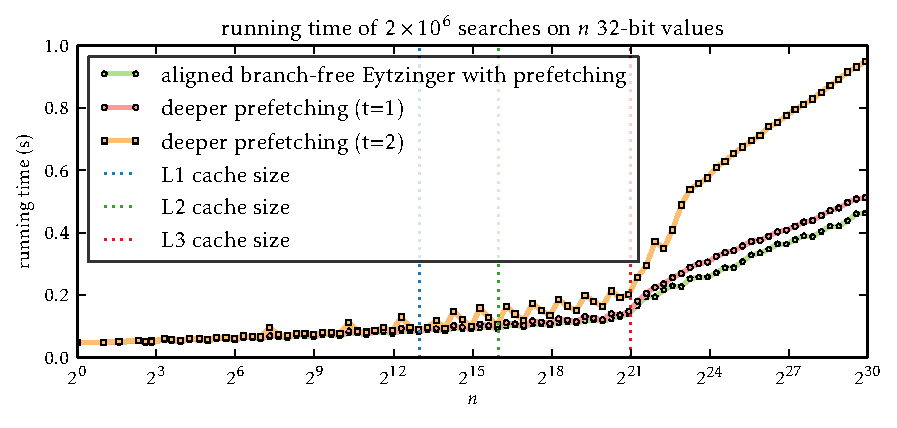
\includegraphics{figs/fetchers-4-i}}
     \centering{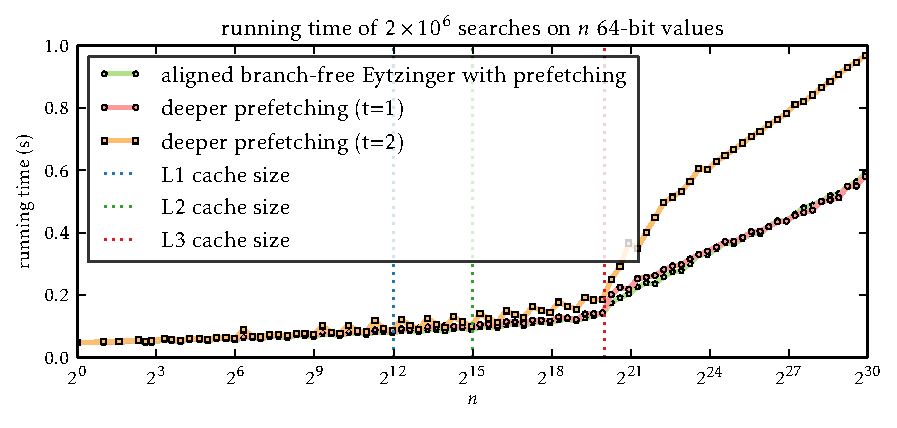
\includegraphics{figs/fetchers-8-i}}
     \centering{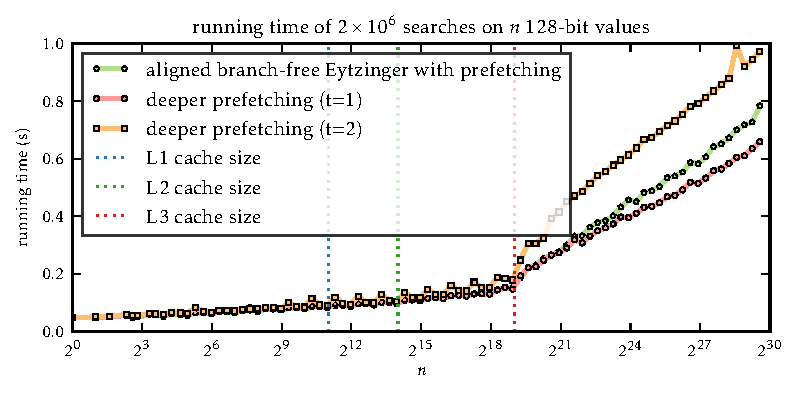
\includegraphics{figs/fetchers-16-i}}
   \caption{The effects of deeper prefetching in the Eytzinger search algorithm.}
   \figlabel{deeper}
\end{figure}

\subsection{The $k(B+1)$-tree}

Our extended I/O model also suggests a \emph{simulation}, in the sense
that, for any $k\le W$ one can load $k$ cache lines in $L+r(k)$ time
units, where $r(k)$ is the time it takes to issue $k$ prefetch requests.
By doing this, one can simulate a model with cache line width $B'=kB$
and latency $L=L+r(k)$.

This immediately raises the question of whether this simulation leads to
a useful data structure.  To test this, we implemented a $(kB+1)$-tree
where, before searching within a node, we first issue $k$ prefetch
commands to load the $k$ cache lines used by that node.  This idea of
using prefetching to get extra-wide nodes ``almost for free'' is the
essential idea used to speed up searches in Chen \etal's prefetching
B$^+$-tree \cite{chen.gibbons.ea:improving}.  \Figref{bktree} shows
the results of implementing this for all $k\in\{1,\ldots,16\}$. The best
choices of $k$ on this machine seem to be $k\in\{6,7,8,9,10\}$.

\begin{figure}
   \centering{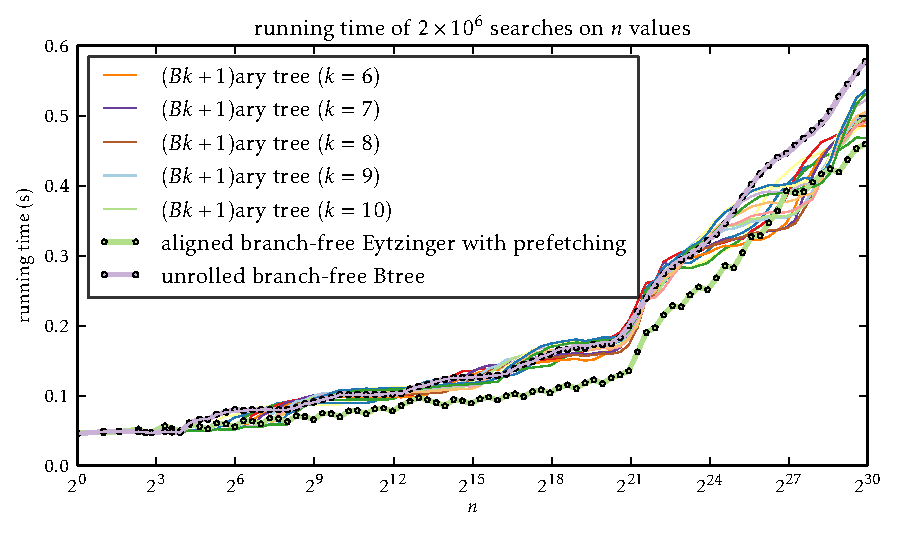
\includegraphics{figs/bktrees-i}}
   \caption{Testing $(Bk+1)$-ary trees}
   \figlabel{bktree}
\end{figure}

These results show that one can, indeed, speedup the Btree layout for some
sufficiently large values of $n$ by using this technique.  This offers
some validation of the extension of the I/O model proposed above.
For some choices of $k$ and some values of $n$, this yields a layout
that is faster than the Eytzinger layout.

Unfortunately, the $(Bk+1)$-tree requires more parameter-tuning than the
Eytzinger layout and only beats the Eytzinger layout for a limited range
of $n$.  This latter fact is because $(Bk+1)$-trees have extremely high
arity; the fastest versions have internal nodes with 97 ($k=6$) to 161
($k=10$) children per node. This makes them inefficient except when the
bottom level is nearly full or nearly empty, i.e., when $n$ is close to
a power of $(Bk+1)$.  This is what causes the large oscillations that
appear in \figref{bktree}.

\section{Further Experiments}
\seclabel{experiments}

In this section, we discuss further experiments that consider the effects
of multiple threads, larger data items, data sizes that exceed the size
of the translation lookaside buffer, and experiments on machines other
than the Intel 4790K.

\subsection{Multiple Threads}

Since the Eytzinger search moves more data from RAM into cache,
it uses more memory bandwidth.  This works because, as discussed in
\secref{bandwidth}, latency, not bandwidth, is the bottleneck; the
bandwidth far exceeds the cache line width divided by the latency.
However, when multiple threads are performing searches in parallel they
could---in theory---saturate the bandwidth.

Figure~\ref{fig:threads} shows the results of tests
using 2, 4, and 8 threads.  In these tests, the array layout is created
and $k$ threads are created, each of which performs $2\times 10^6$
random searches (each thread seeds its own random number generator
with its own unique seed).  The main thread then joins each of these
threads. The total time measured is the time elapsed between (before)
the creation of the first thread until (after) the last thread completes.

\begin{figure}
   \centering{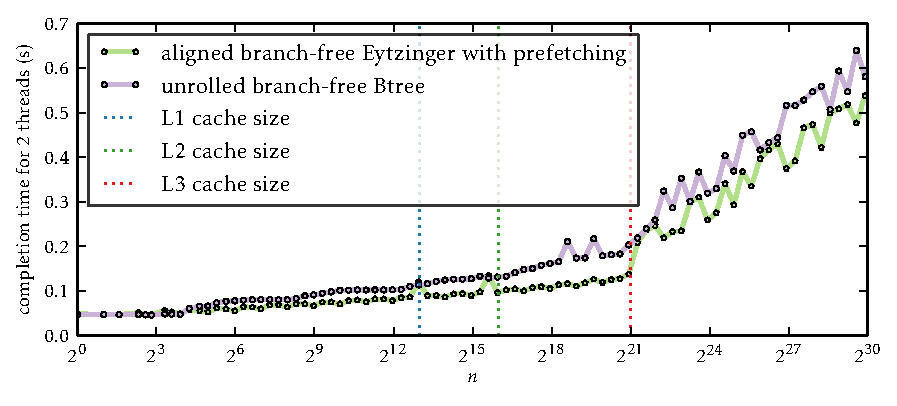
\includegraphics{figs/threads2}}
   \centering{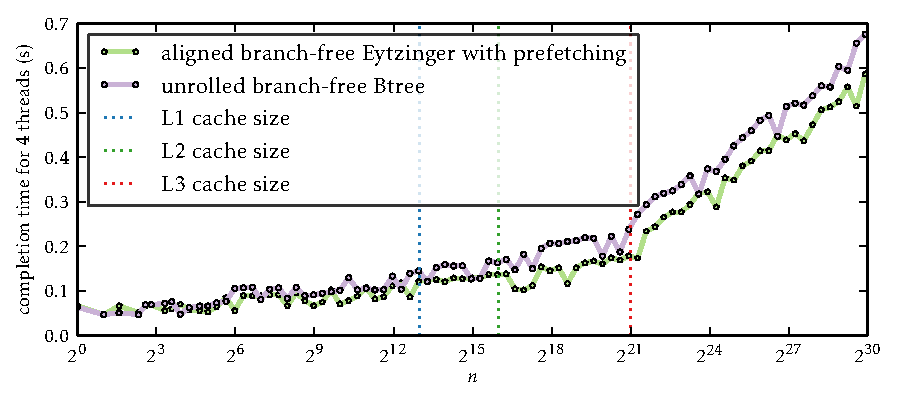
\includegraphics{figs/threads4}}
   \centering{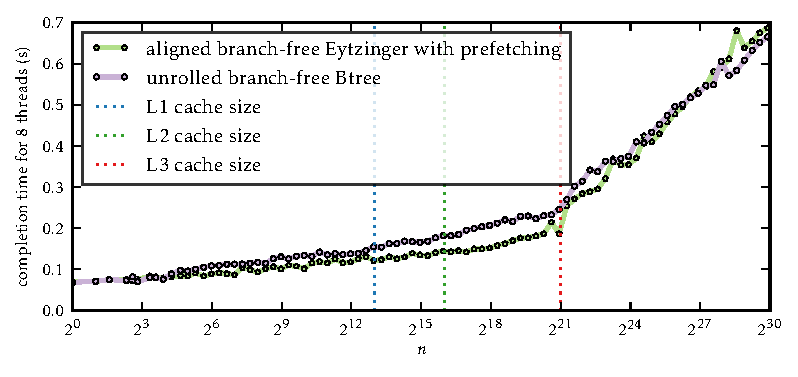
\includegraphics{figs/threads8}}
   \caption{The performance of searches with two, four, and eight threads.}
   \figlabel{threads}
\end{figure}

These graphs show that, although the performance gap narrows, the
Eytzinger layout continues to outperform the other layouts even with four
threads simultaneously searching the array.  With eight threads and very
large values of $n$ the two become equally matched.  We did not test
more than eight threads since this seems unrealistic; the Intel 4790K
has only 4 hyperthreaded cores, which appear to the operating system as
8 CPUs. It does not make sense to run more than 8 computation-intensive
threads simultaneously.


\subsection{Larger Data Items}

\Figref{larger} shows timing results for 8-byte (64-bit) data items and
16-byte (128-bit) simulated data items.  Each simulated 16-byte datum is a
structure that contains an 8-byte unsigned integer and 8-bytes of padding.

In these experiments, the $(B+1)$-trees use values of $B=8$ and $B=4$,
respectively. Similarly, the Eytzinger search algorithm prefetches the
8 virtual nodes that are 3 (for 8-byte data) and the four virtual nodes
that are 2 (for 16-byte data) levels below the current node.

\begin{figure}
   \centering{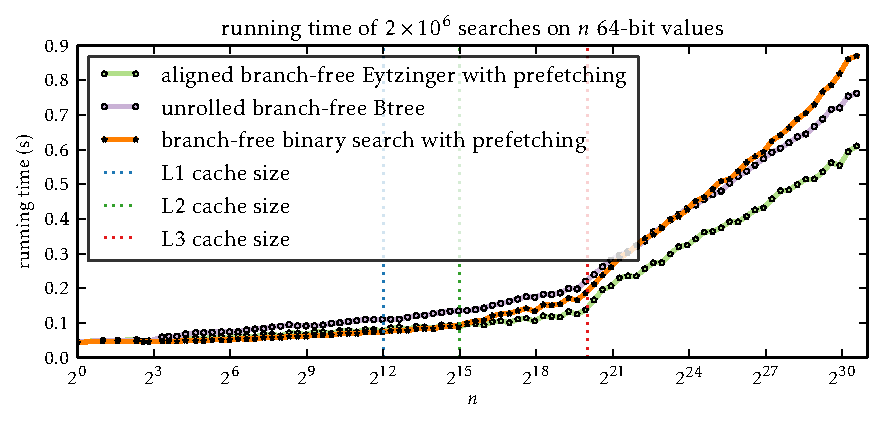
\includegraphics{figs/64bit}}
   \centering{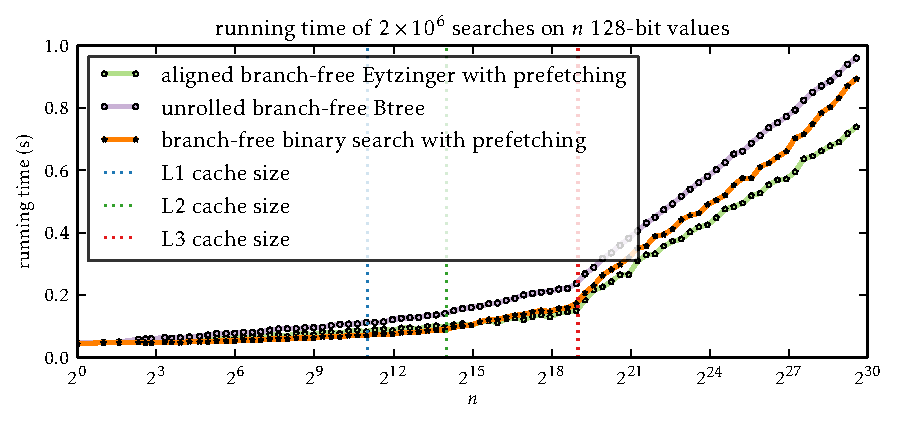
\includegraphics{figs/128bit}}
   \caption{The performance of algorithms on 64-bit and 128-bit data.}
   \figlabel{larger}
\end{figure}

It is worth noting that, in both these figures, the largest value of
$n$ corresponds to approximately 12GB of data. These figures show that
our conclusions hold also for larger data items; the branch-free search
with prefetching in the Eytzinger layout remains the method of choice.
Indeed, as the size of individual data items increases, Eytzinger becomes
a better and better choice.

\subsection{Other Machines}
\seclabel{other-machines}

With the exception of \figref{sorted-atom}, the results presented here are
running times on a single machine with a single memory configuration.
In order to validate these results across a wider variety of hardware,
we also ran a set of experiments on a number of hardware platforms. We
did this by first running experiments on machines we had access to and
then by asking for help from the Internet.

After being surprised by the performance of the branchy
Eytzinger implementation in our own initial experiments
on a handful of machines, we posted to \texttt{reddit}
asking for help testing our initial implementations on more 
hardware.\footnote{\url{https://www.reddit.com/r/compsci/comments/35ad8d/alternatives_to_sorted_arrays_for_binary_searching/}}
This story made the rounds of the usual hacking websites
and, within two weeks we had received testing results
for over 100 different CPUs.  These results are available
online\footnote{\url{http://cglab.ca/~morin/misc/arraylayout/}} and,
overwhelmingly, they showed that our branchy implementation of Eytzinger
search was faster, or at least as fast as our branchy implementation
of Btrees.  It was then that we started micro-optimizing our code to
help understand the reason for this, which led to the conclusions in
the current paper.

The implementations studied in the current paper have been
refined significantly since our initial round of Internet
experiments, so we went back to the Internet for a second
round of experiments, which we are also keeping track of
online.\footnote{\url{http://cglab.ca/~morin/misc/arraylayout-v2/}}
This data is still arriving but in the vast majority of cases so far,
the conclusions agree with those we obtained on the Intel 4790K.  There are two notable exceptions:
\begin{enumerate}
\item With the Atom family of processors, the branch-free code is
typically faster than the branchy code over the full range of values
of $n$.  As discussed in \secref{sorted-discussion}, this is due to
fact that the Atom processors do not perform speculative execution so
the branchy code does not obtain the benefit of implicit prefetching.

\item With some processors (the AMD Phenom II, Intel Celeron J1900,
and Intel E3-1230 are examples) the code that does explicit prefetching
is much slower, especially for smaller values of $n$.  This seems to
be due to executing prefetch instructions that attempt to prefetch
data outside the input array.  Although the documentation for the
\mintinline{c++}{__builtin_prefetch()} instruction specifically
allows prefetching invalid addresses, this seems to cause a significant
performance hit on these processors.  On such architectures, a work-around
is to use a bit-mask to ensure that we never prefetch an address outside
the input array.\footnote{Specifically, we take the bitwise AND of the
prefetched index and $2^{\lfloor\log n\rfloor}-1$.}

\begin{figure}
    \begin{center}
      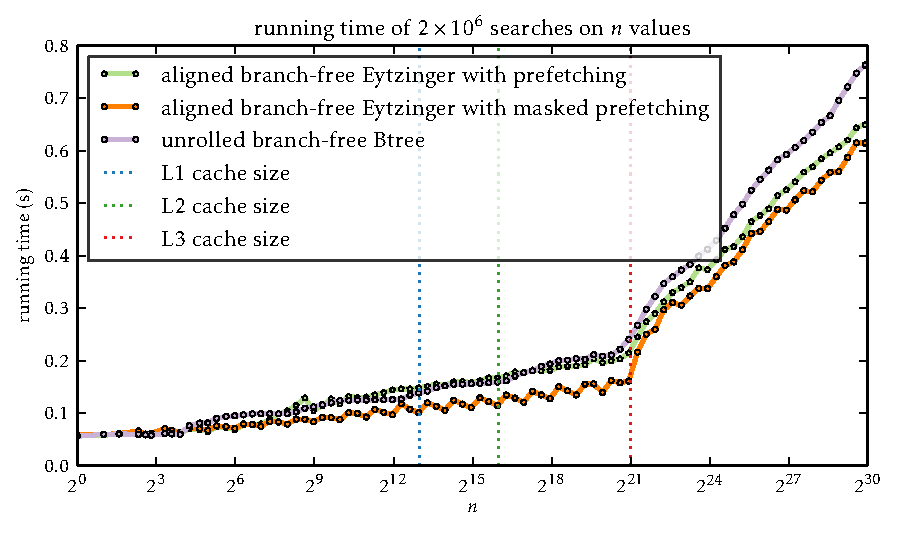
\includegraphics{figs/masking-i}\\[1em]
      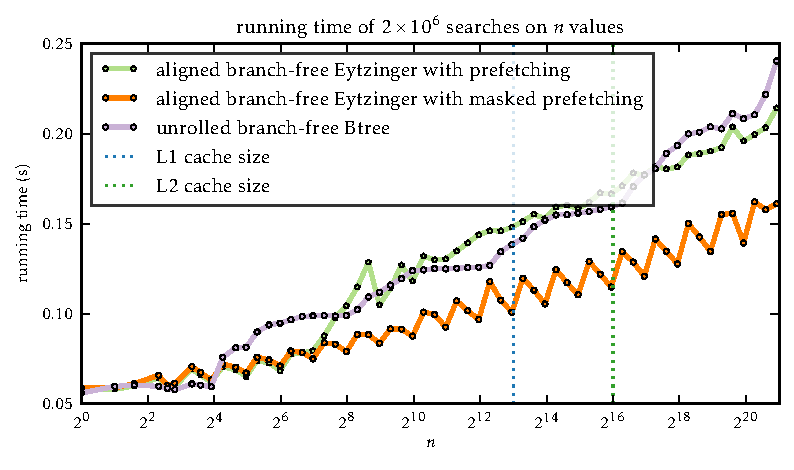
\includegraphics{figs/masking-ii}
   \end{center}
   \caption{Using masking on the Intel E3-1230 to prevent out-of-bounds prefetches.}
   \figlabel{masking}
\end{figure}

\figref{masking} shows the results of using this workaround on the
E3-1230. Using a mask results in reliably fast performance.  We also ran
the same test on the Intel 4790K (see \figref{masking-ii}), and the use
of the mask had almost no impact on performance.  Thus, for reliably
fast code across the largest number of architectures using a mask to
prevent out-of-bounds prefetches seems advisable.
\begin{figure}
    \begin{center}
      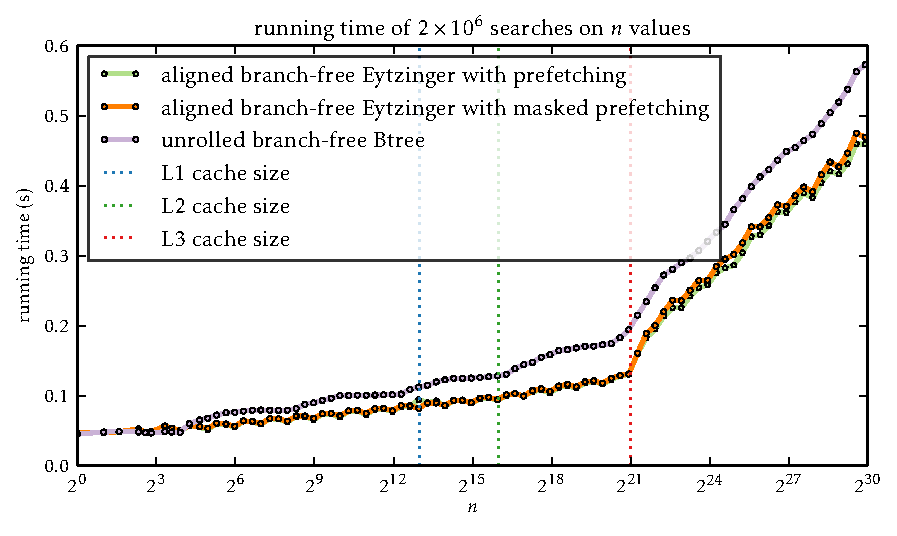
\includegraphics{figs/masking-iii}\\[1em]
      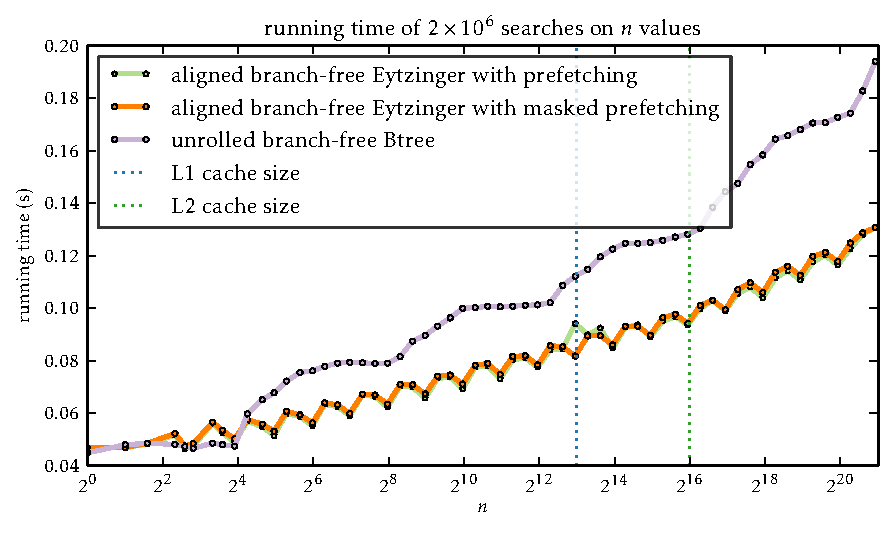
\includegraphics{figs/masking-iv}
   \end{center}
   \caption{Masking prefetches on the Intel 4790K has negligible impact on performance.}
   \figlabel{masking-ii}
\end{figure}

\end{enumerate}

\section{Conclusions and Future Work}
\seclabel{conclusions}

We have compared the relative performance of four memory layouts for
ordered arrays and the algorithms for searching in these layouts.

\subsection{Eytzinger is Best}
Our conclusion is that, for the fastest speed across a wide-variety of
array lengths, an Eytzinger layout and a branch-free search algorithm with
explict prefetching is an excellent choice.  For reliable performance
across a wide variety of architectures, we recommend the variant that
uses a bit mask to prevent prefetching out of bounds.

Not only is searching in an Eytzinger layout fast, it is simple and
compact to implement: Counting semicolons, the Eytzinger search code
consists of 5 lines of code, whereas the fastest Btree code is 19 lines
plus a separate inline subroutine for the inner search.  If we look at
the compiled code, the Eytzinger code contains 26 assembly instructions
and the Btree code contains 78.

Our conclusion is contrary to our expectations and to previous findings
and goes against conventional wisdom, which states that accesses to
RAM are slow, and should be minimized.  A more accurate statement, that
accounts for our findings, is that accesses to RAM have high latency and
this latency needs to be mitigated.  This was formalized in \secref{model}
and the resulting computational model does have some predictive power:
It lead us to deeper prefetching in the Eytzinger search algorithm and
the $(Bk+1)$-tree, which behave more or less as the model predicts.

Practically speaking, this work opens up a whole class of algorithms
and data structures that may be simpler to implement and faster in
practice.  This raises our first open question:

\begin{op}\oplabel{other-problems}
  Can memory request pipelining be used to design faster algorithms for
  other problems?
\end{op}

An obvious candidate to consider in the context of
\opref{other-problems} is the problem of sorting where the
heap-sort algorithm \cite{floyd:algorithm,williams:algorithm},
which already uses the Eytzinger layout, is an obvious starting
point. Scouring the internet, we have only been able to find one
implementation, due to Piotr Tarsa, of heap-sort that makes use of
prefetching, and it only prefetches one level deep.\footnote{See
the files labelled \url{sortalgo/sortheap*cascading*.hpp} in
\url{https://github.com/tarsa/SortingAlgorithmsBenchmark/}}

\subsection{For Big Data, Branchy Code can be a Good Prefetcher}

Today, no computer science research paper is complete unless it says
something about big data.  For small data sets, micro-optimizations
such as replacing branching with conditional instructions can produce
significant improvements in running-time.  For instance, our branch-free
implementation of binary search is about twice as fast as the branchy
implementation for $n<2^{16}$ (refer to \figref{sorted-iii}).

However, as the amount of data increases beyond the size of the
various processor caches, the branchy implementations become faster.
Even for binary search, which represents the worst possible case for
branch prediction, the branchy code eventually outperforms the branch-free
code by an increasing margin (refer to \figref{sorted-iv}).

Our experiments show that this speedup is a result of the interaction
between a long processor pipeline, speculative execution, and the memory
subsystem.  Indeed, speculative execution acts as a form of prefetching
that can speed up memory access patterns that are far too complicated
for current prefetching techniques.  In extreme cases (like the Eytzinger
layout) the resulting prefetches are perfectly correct even four branches
ahead of the current execution point.

In hardware design, the general idea of using speculative execution
as a prefetching strategy is called \emph{runahead execution}
\cite{mutlu.stark.ea:runahead}.  Our results show that, in a processor
that has speculative execution, one can obtain many of the benefits
of runahead even on processors that do not specifically implement it.
While this may not be news to hardware experts, to the best of our
knowledge, we are unaware of any algorithms (or even implementations)
that deliberately make  use of it.

Our results also show
that one has to be very careful with
micro-optimizations.  Optimizations that offer great speedups on small
or moderate-sized inputs can create great slowdowns on large inputs.
For instance, if we compare branch-free versus branchy binary search for
$n=2^{16}$, we find that branch-free binary search is about twice as fast.
However, for $n=2^{30}$, branch-free binary search is about 45\% slower.

%\subsection{In-Place Algorithms for Moving Between Array Layouts}
%
%Finally, we finish with one algorithmic question motivated by our work.
%Since sorted order is what is commonly used in current applications,
%it would be useful to have efficient in-place algorithms to convert from
%sorted order to and from other memory layouts.
%
%\begin{op}
%  Is there a linear time in-place algorithm that converts a sorted array
%  into an array stored in the Eytzinger layout?
%\end{op}
%
%As a starting point we note that, when $n$ is a power of two, there
%is such an algorithm.  In this case, we can use an existing in-place
%algorithm to partition the array into all the odd indices followed
%by all the even indices (this is called an \emph{unshuffle} operation
%\cite[Section~7]{ellis.markov:in-situ}). We can then recurse on the first
%half of the array. This takes linear time and, at the end of this process,
%the array is laid out in Eytzinger order.  Generalizing this algorithm
%to the case where $n$ is not a power of two seems non-trivial.

\section*{Acknowledgements}

We are grateful to  Gerth Brodal, Rolf Fagerberg, and Riko Jacob who
kindly made their source code available to us. However, for a variety
of reasons, most of which have to do with the 12 years that have elapsed
since it was written, we found it impossible to use as a starting point
for our own code.

We are also grateful to the many people who responded to
our online calls for help in testing these algorithms.
Unless they have requested otherwise, their names are
listed on the website we are using to keep track of timing
results.\footnote{\url{http://cglab.ca/~morin/misc/arraylayout-v2/}}


\bibliographystyle{plainurl}
\bibliography{arraylayouts}

\end{document}


